\chapter{光的反射和折射}
\minitoc[n]
\section{教学要求}
    本章讲述几何光学知识,包括两部分内容:一部分是几何
光学的基本规律,讲述光的反射定律和折射定律;另一部分是
运用基本规律来研究平面镜、球面镜、棱镜和透镜等基本光学
元件,这些元件在成像和控制光路方面各有其自身的规律和
特点.学习这些知识,可以便我们认识自然界和生活中的许
多光现象,理解基本光学元件的作用和光学仪器的原理.因
此,这一章知识具有实际意义.

全章教材分为五个单元.一、二节为第一单元,讲述光的
直线传播和光速.三、四节为第二单元,讲述光的反射和平面
镜、球面镜.五—八节为第三单元,讲述光的折射、全反射和
棱镜.九—十二节为第四单元,讲述透镜知识.十三、十四节
为第五单元,讲述眼睛、显微镜和望远镜的构造和成像原理.

本章教材相当大一部分内容是在复习初中知识的基础
上,进一步扩大、加深和提高的.光的直线传播、光的反射等
知识,是复习性的教材.光的折射则在初中学过的知识基础
上予以提高,引入了折射定律和折射率的概念,是进一步学习
棱镜、色散、透镜的知识基础.透镜是许多光学仪器的主要元
件,掌握透镜成像的规律,可以理解一些助视仪器的成像原
理.所以,光的折射和透镜成像是本章教学的重点.

这一章的教学要求是:
\begin{enumerate}
\item 了解光在同一媒质中沿直线传播的性质,会用光的
直线传播解释有关的现象.知道光在真空中的速度.
\item 掌握光的反射定律,会用反射定律解释有关的现象.
掌握平面镜成像的原理和规律.了解凹镜对光的会聚作用和
凸镜对光的发散作用,了解它们的成像规律,
\item 掌握光的折射定律和折射率的概念,了解媒质的折射
率与光速的关系;会用折射定律解释简单的现象.
\item 理解光的全反射现象,掌握临界角的概念和发生全反
射的条件,了解全反射现象的应用.
\item 了解棱镜对光的偏折作用和光通过棱镜后的色散
现象.
\item 了解凸透镜对光的会聚作用和凹透镜对光的发散作
用.了解透镜的主轴、光心、焦点和焦距,掌握透镜成像规律、
成像作图法和成像公式.
\item 了解眼睛、显微镜和望远镜的基本构造和成像原理,
了解近视眼和远视眼以及眼镜的作用.
\end{enumerate}

虽然学生每天都接触光现象,但是却不能直接看到光的
传播路径,讲解光的反射、折射和全反射,要做好演示,让学
生看到光的传播路径,以利于揭示规律,加深印象,同时也可
以提高学生的学习兴趣.

在几何光学的教学中,研究成像是一个重要的问题,要让
学生了解成像规律和所成像的虚实.但是要注意,不要机械
地记忆什么镜成什么像,而要着重让学生从根本上弄清实像
和虚像的含义,掌握分析成像的规律和成像性质的方法.

在反射和折射现象中光路的可逆性对分析实际问题很有
用.教学中要通过具体例子让学生领会到这一点.

媒质的折射率是个重要的概念,要让学生掌握绝对折射
率的概念,为了使学生了解媒质的折射率总是相对于另一种
媒质而言的,教材介绍了相对折射率,教学中不要求把相对
折射率与绝对折射率的关系作为讲述重点,也不要求利用相
对折射率进行计算.

学生对于全反射现象是比较生疏的.教学中应通过演示
让学生认识这个现象,理解产生全反射现象的条件.在演示
时,还应引导学生注意观察光强分布的变化情况,这对于正确
理解全反射现象是有帮助的.光导纤维是全反射现象的应
用,教学中可根据实际情况,向学生介绍这一新技术的发展情
况,以开阔学生的眼界.

透镜是许多光学仪器的重要元件.在透镜成像的教学
中,要求学生会用三条特殊光线求出像的位置、大小和倒正,
判断像的虚实.对于透镜成像公式,应使学生能独立地把它
推导出来,知道什么情况下$f$取正值,什么情况下$f$取负值,
并能根据$v$的正负,判断出像的虚实、倒正和位置.

最后一个单元介绍眼睛、显微镜和望远镜.讲眼睛时,主
要从物理方面讲解眼睛的成像原理,眼睛的调节以及近视眼、
远视眼和眼镜的作用,不要过多地牵涉与生理机制有关的内
容,对于显微镜和望远镜,主要学习它们的基本构造和成像
原理.要求学生能看懂光路图,了解视角放大的情况.如果
有条件,最好在教学中能结合望远镜和显微镜的实物来讲解,
并介绍一些使用和维护方面的知识.

\section{教学建议}
\subsection{光的直线传播和光的速度}
光的直线传播是几何光学的基础,应通过演示实验让
学生看到光传播的路径.演示内容应包括:
\begin{enumerate}
\item 光在同一种均
匀媒质中沿直线传播;    \item 光到达两种媒质的界面,发生反射和
折射;    \item 条件较好的学校还可演示光在非均匀媒质中传播时
光线发生弯曲的现象(为阅读教材“海市蜃楼”做准备).
\end{enumerate}


光线是几何光学的最基本的概念之一,它为应用几何
学的方法研究光的传播奠定了基础,光的反射定律和折射定
律等都是应用光线的概念来表述的,要使学生理解:
\begin{enumerate}
\item 光线
的概念建立在光的直线传播的基础上,所以,作图时画光线必
须要有表示光传播方向的头.    
\item 光线和光是有区别的,光
线只代表了光的传播方向,并不是实际存在的东西,而光是实
际存在的.    
\item 有时用光线代表很窄的平行光束的传播路径,
从这个意义上讲,光线是光束的抽象;有时又用两条光线代表
一束光束,这两条光线表示光束的边缘,也表示出光束的会
聚、发散或平行的性质.
\end{enumerate}

要注意应用几何学的方法研究与光的传播有关的实
际问题.在对影、本影和半影等问题进行分析时可参考下面
五点逐步深入:
\begin{enumerate}

\item 点光源发出的光照到不透明物体上,在物
体背后的光屏上可以看到光线照不到的黑暗区域——影子.
作出光路图,说明影子的范围;
\item 如果物体大小是已知的,应
用相似形的关系可以说明影子的大小决定于点光源、物体和光屏的相对位置;\item 利用发光面较大的面光源代替点光源,
说明本影和半影的概念;
\item 面光源的线度大于物体时,移动
光屏的位置,讨论屏上影的情况,说明本影、半影等概念的关
系.
\item 观察者处于图5.1中$A$、$B$、$C$、$D$等不同位置时看面
光源$PQ$, 见到的现象会不同.通过以上分析,可以为学生认
识日蚀或月蚀等现象、解答课本练习一第2题打下基
础,教学时应着重引导学生体会几何光学的研究方法:从光
传播的基本定律出发,做出光路图,运用几何学的方法研究
有关线段、角度等量的关系.
\end{enumerate}

\begin{figure}[htp]
    \centering
    \includegraphics[scale=.6]{fig/5-1.png}
    \caption{}
\end{figure}

光的速度是物理学中的重要基本常数,为了测量光
速,从十七世纪伽利略开始一直到今天,经过了许多科学家
的努力,测量结果越来越精确.讲述光的速度要结合物理学
史介绍科学家百折不挠、精益求精的探索精神,要重点讲述光
的传播速度虽然很大,但是有限的,分析测量光速实验的设计
思想.伽利略根据$v=s/t$
的原理进行了历史上第一次测光速
的实验,尽管没能测出光的速度来,但是他的实验设计思想却
给人们指出了努力方向,由于光速是很大的,早期测量光速
的方法或者是增大光传播的距离,或者是利用更精巧的办法
准确地测量光传播的时间.

罗默观测木星的卫星蚀,第一次证实了光以有限的速度
传播,用的就是前一种方法.学生理解罗默方法的原理是有
困难的,教材并不要求掌握具体细节,但应使学生理解:虽然
卫星绕木星运动的周期是固定的,但在地球上观测木星的两
次卫星蚀的时间间隔却是不同的,这是由于地球位于公转轨
道上的不同位置时,与木星的卫星间的距离不同.而光以有
限速度传播,从卫星发出的光到达地球时经过的距离不等,因
此,观测到的卫星蚀的时间间隔也就不等.

迈克耳逊用旋转棱镜法测光速,是采用精巧的办法准确
地测量出光传播的时间.他是早期测量光速最准确的科学家.
讲述旋转棱镜法测光速的实验设计思想时,要着重理解光由
光源$S$发出最后到达望远镜$C$中(课本图5.5)所经过
的路径和旋转棱镜能精巧地测量时间的原理,调节八面棱镜
的转速,使光由凹镜反射返回来时八面镜恰好转过$1/8$转,在
望远镜$C$中能看到$S$的像(还可进一步引导学生讨论转速增
加到转过$\frac{2}{8},\frac{3}{8},\ldots$
转的情况).测出转速便可求得光在两
个山峰之间往返一次所用的时间.

近代科学家还提出用其他的实验原理来测量光速.例如
测量激光的频率$\nu$,和波长$\lambda$, 根据公式$c=\lambda\cdot \nu$计算光速,大
大提高了测量的精度.应该要求学生记住真空中光速的近似
值$c=3.00\x10^8\ms$.

\subsection{光的反射}
\subsubsection{反射定律}

反射定律、镜面反射和漫反射在初中讲得
都比较清楚,教材中这部分内容是按照复习旧知识安排的.可
以通过演示光的反射光路、镜面反射和漫反射,再现这些现
象,再进一步采用讨论的方法加深对反射定律的认识.选择
讨论题目要针对学生的具体情况,下列问题可供参考:
\begin{enumerate}
\item 在什么条件下发生光的反射现象?
\item 反射定律的内容为什么一定要包括课本中讲的两条?
    \item 怎样确定反射界面的法线?如
果界面是球面,它的法线是什么?
    \item 发生镜面反射时,反射光
线和入射光线之间的夹角取值范围可能多大?
    \item 漫反射和镜面反射有什么区别和联系?
\end{enumerate}



\subsubsection{光路的可逆性}

光路的可逆性是几何光学的重要原
理之一.要结合反射定律(包括以后的折射定律)理解反射时
的光路(包括折射时的光路)是可逆的.几何光学中的光路(面
镜、棱镜和透镜的光路和成像)都建立在反射定律和折射定
律的基础之上,并且几何光学中的所有光路都是可逆的,应
该注意,物理光学中的光路是不可逆的.

做为一种方法,光路的可逆性可以用来解决一些具体问
题.例如,人眼的视野问题.可以设想在人眼所在的位置处
放一个点光源,求出由该点光源发出的光所能照亮的区域,根
据光路可逆性,在这个区域内的物体发出的光都能到达人眼,
被人眼看到.因此,这个区域是人眼的视野范围.

\subsubsection{平面镜}

平面镜的内容也是在初中知识的基础上讲
述的.讲述的重点放在虚像的概念、虚像的形成以及平面镜
成像的特点上.

虚像的概念及其形成分三个层次讲解:
\begin{enumerate}
\item 在光的直
线传播一节中讲述了根据光的直线传播确定发光点的位置,
这为讲解虚像做了准备、由发光点发出的光向各个方向传播,
可以将其中的任意两条光线反向延长,它们的交点就是发光
点的位置.应该注意,这两条光线必须是同一发光点发出的,
由不同发光点发出的两条光线的交点,在成像问题上没有意
义;
\item 由某一物点$S$发出的、经平面镜反射后的光线进入了眼
睛,人们根据光的直线传播的经验认为这些光线都是由它们
的反向延长线的交点$S'$射来的,好象在$S'$点有一个发光点
一样,$S'$点就是物点$S$的虚像.这里说明了虚像不是光线的
实际交点,是“虚”的,需要借助其他光学仪器(如眼睛)才能观
察到;
\item 组成物体的每一个物点都在平面镜里产生一个虚像
点,这些虚像点的集合就是物体的虚像.教学中要注意培养
学生抽象思维的能力,不仅要从实验现象中看到物体通过平
面镜可以成像,还要学会从理论上分析推理得出像的概念,
再根据反射定律进一步推出物体通过平面镜所成的像是等
大、正立的虚像,物和像对于镜面是对称的.
\end{enumerate}

平面镜的应用包括应用平面镜成像,应用平面镜控
制光路等,在课文中提到了利用平面镜将微小效应放大、潜望
镜的光路图等实例,在习题中安排了平面镜成像,利用激光测
量月球和地球间的距离以及人眼通过平面镜观察的视野范围
等问题.在分析实际问题时要画好光路图,使学生了解几何光
学的研究方法,培养他们灵活应用物理知识解决实际问题的
能力.

\subsubsection{球面镜}

通过演示实验复习凹镜的会聚作用和凸镜
的发散作用,注意从实验观察到的光路出发讲述球面镜的顶
点、主轴、焦点(实焦点和虚焦点)和焦距等概念.进一步理解
课本193页讲述的凹镜和凸镜的实际应用的例子.

近轴光线是球面镜和透镜能成理想像的前提条件,教材
中给出了在近轴条件下,球面镜的焦距$f=r/2$
是为了使学
生对球面镜焦距的大小有一个具体的了解,并不要求深入展
开讨论和证明这个公式.根据反射定律,可以分别画出平行
于主轴的近轴光线和远轴光线经过凹镜反射后与主轴的交
点,如图5.2中的$F$和$E$点,说明球面镜的非近轴光线不能会
聚于一点.实验给出的几条光线能够在焦点会聚仅是近似
的;近似的条件就是入射光线都是近轴光线.为了使远轴的
平行光线也能会聚于焦点,实际应用的大口径凹镜都用抛物
面镜而不用球面镜.
\begin{figure}[htp]
    \centering
    \includegraphics[scale=.6]{fig/5-2.png}
    \caption{}
\end{figure}

球面镜成像是从实验得出的,教材不要求画成像的光路
图,也不要求讲述球面镜成像公式,只是从实验得出物体通过
凹镜可以成放大实像、缩小实像和放大虚像,通过凸镜只能成
缩小虚像的情况 演示实验中要让学生注意观察用光屏能够
接收到实像,而无论把光屏放在什么位置都不能接收到虚像.
这表明实像是反射光线实际会聚而成的;虚像不是反射光线
的实际会聚点,而是光线的反向延长线的交点,这是实像和虚
像的主要区别.


\subsection{光的折射}

折射定律和折射率是本章的重点内容,可以按下述
几个层次安排教学.
\begin{enumerate}
\item 通过演示实验观察光在两种媒质的界面上的折射现
象,观察折射角随入射角的增大而增大的规律,激发学生深入
研究折射角和入射角的关系的学习动机.
\item 分析课本197页表中的实验数据,得出折射定律.
\item 折射定律中的常数决定于两种媒质的性质,引入相
对折射率$n_{21}$·
\item 引入绝对折射率,进而求出相对折射率和绝对折射
率的关系.
\end{enumerate}

\subsubsection{折射定律}

课本结合物理学史讲述了历史上经历了
一千多年,由托勒密到斯涅耳经过许多科学家的努力,从大量
的实验数据中归纳总结出折射定律,教学过程也要从演示折
射现象开始,演示的内容有:
\begin{enumerate}
\item 光达到两种媒质的界面上发生
折射的现象;
\item 折射角随入射角增大而增大的规律;
\item 光由光
疏媒质进入光密媒质向靠近法线方向偏折,光由光密媒质进
入光疏媒质向远离法线方向偏折.
\end{enumerate}
通过演示,使学生获得光
的折射现象的感性认识.在定性实验的基础上,再分析课本
197页表中所给出的实验数据,说明托勒密最初得出的折射
角与入射角成正比的结论是片面的,给出斯涅耳经过深入的
分析得出的折射定律内容.(折射定律现代表述的形式是由
笛卡儿提出的.)

和反射定律一样,掌握折射定律也要注意培养学生的想
象力,要使学生建立起光由媒质I进入媒质II的折射图景.
使学生在理解界面及其法线、入射光线和折射光线,入射角和
折射角等概念的基础上,进一步掌握折射定律.折射定律的
第一点指出了入射光线、折射光线、法线在平面内的大致方
位,第二点定量地确定折射角,确定折射光线的确切方向.

\subsubsection{折射率}

媒质的折射率是由折射定律引入的.教材
从光在两种媒质界面上发生折射的现象入手,引入相对折射
率,并且直接给出了相对折射率和光在两种媒质中传播速度
的关系,然后从光从真空进入媒质发生折射的特殊情况,引
入绝对折射率的概念,并通过折射率和光速的关系,求出相对
折射率和绝对折射率的关系.这部分内容,特别是绝对折射
率和相对折射率的关系,涉及的物理量比较多,初学者较难
掌握,容易造成混乱.教学中应强调$n_{21}$下标的表述及其意
义.讲解公式$n_{21}=\dfrac{n_2}{n_1}=\frac{v_1}{v_2}$时,要和具体的光疏、光密媒质以
及光线的偏折情况相联系.

教学中要注意培养学生的想象力,建立光由媒质I射入
媒质II发生折射的图景,理解其中的平面、直线、角度之间的
关系,进一步寻求入射角和折射角、媒质的折射率及光速之
间的关系,例如,已知水中的光速是真空中光速的$3/4$,光由
空气进入水中,以多大的入射角射入时,反射光线和折射光线
垂直,学生在头脑中建立了光在空气和水的界面上发生反射
和折射的图景之后,就能找到入射角、反射角和折射角间的关
系,求出入射角来.

课本201页讨论的光通过两面平行的玻璃砖发生侧移的
例题,既应用了折射定律分析解决具体问题,又为“测定玻璃
折射率”的学生实验做准备.可以先演示光通过玻璃砖发生平
行侧移的现象,再提出如下问题:
\begin{enumerate}
\item 光线穿过玻璃砖后,为什
么只发生平移而不改变传播方向?
\item 光线平行侧移的距离、方
向决定于什么条件?
\end{enumerate}
让学生自己通过讨论去研究解释这个现
象,寻求例题的解.

\subsubsection{全反射}
 由于学生先接受了光到达两种媒质的界面
上既要发生反射,又要发生折射的现象,要进一步认识在一定
条件下,光到达界面上只发生反射不发生折射的全反射现象
比较困难,学生往往对于发生全反射的条件理解不深刻.教
学中,要使学生在实验的基础上,认识全反射现象,了解发生
全反射的条件.

做演示实验时,要使学生看到光从光密媒质射入光疏媒
质时,折射角大于入射角.随着入射角的增大,折射角也逐渐
增大.当入射角达到某一角度时,折射角达到$90^{\circ}$. 再增大
入射角,就只有反射光线,没有折射光线.通过现象的观察,
使学生了解全反射现象是光由光密媒质射入光疏媒质时,入
射角达到某一特定值以后产生的现象.这有助于使学生弄清
楚“临界角”的含义.

还要使学生理解全反射现象并不违背折射定律.当光从
光密媒质进入光疏媒质时,有$\sin r=\dfrac{\sin i}{n_{21}}$, 而光疏媒质对
光密媒质的相对折射率$n_{21}=\dfrac{v_1}{v_2}<1$, 所以折射角$r$大于入射
角$i$. 当折射角$r=90^{\circ}$时,即使再增大入射角,也不会存
在大于$90^{\circ}$的折射角$r$, 这时就发生了全反射现象.

教学时,可结合实验观察使学生理解临界角的概念,掌
握计算临界角的方法.

为使学生获得全面的认识,在讨论全反射现象时,也可以
分析光由光疏媒质进入光密媒质的情况.通过比较,加深学
生对产生全反射条件的认识.

在演示时,还要注意引导学生观察入射光的能量在反射
光和折射光中的分配随入射角的大小而变化.使学生认识到
发生全反射时,入射光线的能量几乎都被反射回原来的媒质
中,没有光能量进入另一种媒质,因而反射光最强.由此可以
认识生活中的全反射现象,如课本205页讲述的实例,以及使
用光导纤维和全反射棱镜的意义.

\subsubsection{棱镜}
三棱镜对光的偏折作用和色散现象是折射定律的具体应
用,设计如下的教学过程可供参考.

演示单色光通过三棱镜发生偏折的光路,分别演示
棱镜的底面在下方和底面在上方的两种情况,让学生观察现
象,归纳出光过三棱镜总是向底面偏折的结论.

根据折射定律讨论光在三棱镜两个侧面的折射,定
性地说明光通过光密三棱镜向底面偏折的光路.也要提醒学
生注意,如果是光疏三棱镜,光的偏折情况将会怎样?让学生
在做课本练习六第1题时回答.

定性说明偏折角度$\theta$与棱镜的折射率有关.在保持
入射角$i$和棱镜顶角$A$不变的条件下,棱镜材料的折射率越
大,偏折角度也越大.这是由于棱镜的折射率大,在$AB$面
上光的偏折角度也大,也就是$AC$面上的入射角变大.在$AC$
面,由于入射角和棱镜材料的折射率都变大,偏折角度也要变
大.因此总的偏折角度随折射率增大而增大.

演示白光过三棱镜的色散现象,可观察到由色散
产生的彩色光带(连续光谱).要注意引导学生观察色散时光线
的偏折方向以及光谱中不同颜色光的偏折角度.演示时还应
在三棱镜的入射侧面前加红、黄、蓝等不同颜色的滤色片,显示
单色光通过棱镜的偏折情况.可以看到红光偏折最小,蓝光
偏折最大.由此揭示白光包含有各种颜色的色光,不同色光通
过棱镜的偏折角度不同,进而可以解释产生色散现象的原因.

组成白光的各种单色光,对三棱镜的入射角都相同,
但出射时各色光偏折角度不同,这是由于棱镜对于不同色光
的折射率不同造成的,红光的偏折最小,表明棱镜材料对于红
光的折射率最小;蓝光的偏折大,表明棱镜对于蓝光的折射率
较大,要让学生了解媒质对于不同颜色的光的折射率不同,说
明不同色光在该媒质中的传播速度不一样,使学生进一步加
深对折射率的认识.

可结合练习五中的题目讲一讲全反射棱镜.常用的
全反射棱镜是等腰直角三棱镜.在光学仪器中常用它来控制
光路,改变光线的传播方向或使像倒转等.例如,潜望镜中用
全反射棱镜代替平面反光镜,改变光线的传播方向;望远镜中
常用一对全反射棱镜使像的上下和左右都反转,观察者能够
直接看到正立的像.

常用一对全反射棱镜使像的上下和左右都反转,观察者能够
直接看到正立的像.

\subsection{透镜}
这一单元讲述透镜的成像规律,成像作图法和成像公式.
这些内容是本章中重要的基础知识,也是教学的重点.

实验是讲解透镜知识的基础.凸透镜对于光线的会
聚作用,凹透镜对于光线的发散作用,物体通过透镜可以成像
(包括实像和虚像),都是通过实验得出结论的.通过实验建
立起物和像的一一对应关系,为进一步用作图法和公式法研
究物像的关系打好基础,要做好下述演示实验:

平行于主轴的光线通过凸透镜后都会聚于主轴上的
一点;平行于主轴的光线通过凹透镜后变得发散,借助于直尺
看出出射光线的延长线交于主轴上的一点.通过实验的光路
讲述主轴、光心、焦点(包括实焦点和虚焦点)和焦距等概念.

从主轴、光心、焦点的概念分别引出凸透镜和凹透镜
的三条主要光线,再用实验复现这三条主要光线,强化学生的
认识.

通过演示实验复习物体通过凸透镜成像的五种情况
($u=f$时不成像)和凹透镜成像的一种情况.演示过程要注
意:
\begin{enumerate}
\item 利用光屏接收实像,确定实像的位置要注意实验操作的
示范,让学生看到光屏在成像位置附近移动时,像由模糊到清
晰再到模糊的过程.
\item 改变物距的大小应由物距较大逐渐变
为较小,使学生对于凸透镜和凹透镜成像的几种情况有比较
完整的认识,体会研究方法,切忌只孤立地演示成像的几种情
况,而不体现物距(或像距)连续变化的过程.
\end{enumerate}

\subsubsection{成像作图}

透镜成像作图建立在物体通过透镜可以
成像的实验基础之上,物体上的每一个发光点都对应着一个
像点,即由物点发出的光线经过透镜折射后,所有出射光线,包
括三条主要光线,都汇交于它对应的像点.课本安排练
习九第1题的目的就是为了加深这个认识,为了确定像点的
位置,可以在这些光线中任意选取两条出射光线求得交点,选
用三条主要光线中的两条比较方便.同样,确定物点的位置,
也可求出与像点相应的任意两条入射光线的交点.这样,可以
使学生认识物点和像点的意义,认识成像作图的基本出发点,
正确理解作图方法,避免得出只有三条主要光线才能成像的
错误印象.

教学中要注意示范,使学生养成作图规范的良好习惯,作
图规范包括:每条光线在透镜折射前后都应标出表示光线行
进方向的箭头;正确绘出透镜的符号,标注光心、焦点以及物
和像的位置和正倒;分清图中的实线和虚线.

教学中还要注意:
\begin{enumerate}
\item 采用对比的方法区别凸透镜和凹透镜三条主要光线
的不同点.学生对凹透镜的三条主要光线往往掌握不好,其
主要原因是对于虚焦点的概念和位置理解不深刻,混淆了凹
透镜和凸透镜对光线的作用.
\item 强调物点是透镜的入射光线的出射点,像点则是上
述入射光线经透镜折射后的出射光线或其延长线的交点,不
是随意两条光线的交点,学生往往不注意这点而造成错误.
\item 利用作图法确定物像关系,要和物体通过透镜成像
的情况相联系,许多实际问题往往是在分析成像情况做出判
断后才能正确做图.
\end{enumerate}

教材不要求讲述副光轴和焦平面、副焦点的知识,一般情
况只做主轴外物点的成像光路图,对于垂直于主轴的物体,
它的像也垂直于主轴,可以只求主轴外物点的像,成像光路如
图5.3所示,为了确定主轴上物点的像的位置,可以借助于
过该点的垂直于主轴的物体的成像作图,求得它的像点.
\begin{figure}[htp]
    \centering
    \includegraphics[scale=.6]{fig/5-3.png}
    \caption{}
\end{figure}

利用几何作图说明实物通过凸透镜和凹透镜成像的几种
情况,如图5.4、图5.5所示,可以看到,实像和虚像都是由物
点发出的光经透镜(也包括面镜等其它光学元件)后的出射光
线的交点.物点和像点是一一对应的.实像点是出射光线的实
际交点,可以用光屏来接收,通过光屏的漫射作用,人眼可从
各个方向观察到它;虚像是出射光线延长线的交点,只能由人
眼或其他光学仪器来承接.
\begin{figure}[htp]
    \centering
    \includegraphics[scale=.6]{fig/5-4.png}
    \caption{}
\end{figure}

\begin{figure}[htp]
    \centering
    \includegraphics[scale=.6]{fig/5-5.png}
    \caption{}
\end{figure}

\subsubsection{成像公式}

在几何作图的基础上推导成像公式的思
路是:
\begin{enumerate}
\item 由几何作图给出物像之间存在的一一对应的关系,寻
求物距$u$、像距$v$和焦距$f$间的关系式.
\item 在透镜成像的光
路图中,$u$, $v$, $f$都是主轴上的量,利用相似三角形的几何关系
推得透镜成像公式和放大率公式.
\item 先按照凸透镜实物成实
像的情况推导成像公式,然后引入符号规定,把公式推广到凸
透镜成虚像,凹透镜成虚像的情况,为了使学生信服,在练习
题中安排了证明透镜公式也适用于凹透镜成像.
\end{enumerate}

成像公式$\dfrac{1}{u}+\dfrac{1}{v}=\dfrac{1}{f}$
和放大率公式$m=\dfrac{A'B'}{AB}=\dfrac{v}{u}$
配合使用,既可以确定物体成像的位置,并由像距$v$的正负判断像的
实虚和倒正,也能确定像的放大或缩小的情况;利用这两个公
式还可以讨论物体经过透镜成像的各种情况.课本练
习十第2题就是用公式讨论物体成像的情况,讨论的结果和
作图法得出的结果一样,也跟实验结果一致.

应用透镜成像公式研究物和像的关系是教材的重点.在
使用公式计算时要让学生注意:凸透镜的焦距$f$取正值,凹
透镜的焦距$f$取负值;物距$u$总取正值;实像的像距$v$取正
值,虚像的像距$v$取负值.计算时,要按照正确的符号规则将
已知量的值代入公式,便可得到正确的结果.如果计算出来
的$v$是负值,则表示所成的像是虚像;$f$是负值,表示所用的
透镜是凹透镜.

放大率公式中的$m$总是正值,即$m=|v|/u$.
对于实物成实像的情况,由于$v>0$, 所以$m=v/u$; 对于实物成虚像的情况,
由于$v<0$, 所以$m=-v/u$. 

根据公式讨论透镜成像问题要和成像的光路图结合起
来.按照符号规则,$u$、$v$、$f$都是代数量,有正有负.但是,在从
光路图中线段的几何关系寻找$u$、$v$、$f$各量间的代数关系时,
把图中的几何线段都看作是正值比较方便.因此,与表示凹透
镜焦距的线段对应的代数量可用$-f$, 与表示虚像像距的线段
对应的代数量可用$-v$. 这样在讨论过程中就不会发生选错
符号的问题了.具体例子可参看练习十第1题的解答.下
面再举一例:

某物体通过透镜成放大到3倍的正立像.已知物和像的
距离是12厘米.那么使用的是什么样的透镜?透镜的焦距是
多大?

根据已知条件,这是属于凸透镜成虚像的情况,$v<0$, 与
光路图(图5.6)中表示物距的$OB'$对应的代数量为$-v$.
\begin{figure}[htp]
    \centering
    \includegraphics[scale=.6]{fig/5-6.png}
    \caption{}
\end{figure}

根据物、像关系和放大率公式有:
\[\begin{cases}
    -u-v=12\\
    m=\dfrac{-v}{u}=3
\end{cases}\]
解方程组可得$u=6$厘米,$v=-18$厘米.将$u$、$v$数值代入成
像公式得$f=9$厘米.

课本224页的例题,是应用公式法来研究物像关系.题
目所述的求焦距的方法,是实验室中测量焦距的常用的较准
确的方法.由于这种方法在学生实验中要用到,因此教学时
应使学生理解公式的推导过程,弄懂公式的意义.

\subsection{透镜的应用}
这一单元讲述眼睛、显微镜和望远镜等光学仪器,作为透
镜基础知识的应用.

\subsubsection{眼睛}

眼睛的构造相当于一架精巧的焦距可变的照
相机.讲述时应注意以下几点:

视觉的形成:通过眼球的屈光作用(相当于凸透镜
的作用),物体在视网膜上所成的倒立缩小的实像,刺激眼睛
的感光细胞,再经过神经系统的综合分析作用形成视觉.

眼睛的调节:通过晶状体的弯曲程度来改变眼球的
焦距,使不同距离的物体都能在视网膜上成像.这里要注意
阐明视力范围的远点、近点和明视距离的概念.

近视眼和远视眼的视力范围和正常眼不同,是由眼
睛的屈光系统不正常造成的.通常以眼睛的远点来判断屈光
是否正常,正常眼的远点在无限远处,近视眼的远点在眼前
的有限距离.远视眼所成的像落在视网膜后.

配带眼镜可以矫正近视眼和远视眼.配戴凹透镜可以使
像点后移,配戴凸透镜可以使像点前移.通过演示实验显示
眼镜的矫正作用,使学生得到直观的认识.

有人认为,明视距离的远近是远视眼和近视眼的标志,这
是不科学的.因为明视距离与人的习惯等因素有关.近视眼
和远视眼都具有调节能力,不能准确地测量它们的明视
距离,而且用明视距离也不能准确地表达眼睛的屈光是否
正常.

\subsubsection{显微镜和望远镜}
放大视角扩大眼睛的观察范围是讲述显微镜和望远镜
的主线.这些助视光学仪器做为透镜知识的应用,应着重讲
述它们的构造、成像原理和成像光路图.

显微镜是学生比较熟悉的光学仪器,生物课中学生
曾用它观察微小物体的切片.可以结合“组成显微镜模型”的
学生实验进行教学,让学生自己先预习,再动手做实验,通过
实验了解显微镜的构造,掌握显微镜的成像原理和光路图,理
解使用显微镜怎样达到放大视角的目的.最后应结合实
验说明实际显微镜的构造,讲解使用和调整显微镜的
知识.

望远镜是用来观察远处大物体的助视光学仪器,教
材重点讲述开普勒望远镜的构造、成像原理和光路图.讲解
课本图5.54开普勒望远镜原理图时,应向学生说明
射入物镜的三条平行光线来自远处天体上的同一点,而不是
来自天体上的不同点,目镜所成的虚像的位置应在远处,以免
学生误解.要帮助学生理解望远镜的光路,说明望远镜放大
视角的作用.眼睛通过目镜观察物体虚像的视角大于人眼直
接观察物体的视角,这就好像把物体从远处“拉近”一样.应注
意望远镜只放大视角,并不是得到比物体放大的虚像,实际上
所成的虚像要比物体本身小.

课本还介绍了牛顿反射式望远镜,用大口径的凹镜代替
凸透镜做物镜(课本图5.55反射式望远镜原理图),
反射光线在会聚到焦点以前被平面镜反射,形成实像.通过
目镜再观察这个实像,同样起到放大视角的作用.

条件较好的学校还可以在课后介绍伽利略望远镜,伽利
略望远镜是意大利物理学家伽利略在1609年发明的.它的
物镜是凸透镜,目镜是凹透镜.通过望远镜观察到的像是正
立的.简单的观剧镜和儿童玩具望远镜都是伽利略望远镜.
课本上没讲伽利略望远镜是为了避开虚物成像和副光轴的
问题.

显微镜和开普勒望远镜都是由两个凸透镜组成,除
了显微镜的目镜和物镜的焦距都比望远镜的小之外,还可按
下表所列内容进行比较.

\begin{center}
\begin{tabular}{cp{.4\textwidth}p{.4\textwidth}}
    \hline
   & 显微镜&    望远镜\\
    \hline
    观察对象&近处微小物体&    远处的大物体\\\hline
    构造&物镜焦距$f_1$较小,目镜焦距$f_2$较大,物镜和目镜的距离大于$f_1+f_2$  &
    物镜焦距$f_1$较大,目镜焦距$f_2$较小,物镜和目镜的距离等于$f_1+f_2$\\\hline
    成像特点&物镜成放大实像于目镜的焦距以内,目镜成放大虚像于明视距离处 &
    物镜成缩小实像于焦点附近,目镜成放大虚像于远处 \\
    \hline
\end{tabular}
\end{center}

\section{实验指导}
\subsection{演示实验}

本章的许多演示实验都需要显示光束传播的路径.
显示光束的路径通常用下述两种方法:
\begin{enumerate}
\item 利用微小颗粒对光
的散射.例如,光束通过烟箱,由于烟雾对光的散射,能够显
示出光束行进的路径;
\item 利用光屏的漫反射作用.例如,光束
掠射过光屏,光屏表面对光束的漫反射,显示出光束传播的
路径.
\end{enumerate}

显示光的传播路径的光束应是细窄的平行光束.平行光
源通过一条或几条狭缝后,便得到一束或几束很窄的平行光
束.实验室中可供选择的平行光源有:
\begin{enumerate}
\item 用平面镜引入一束
太阳光做为平行光源.它的优点是比较简单,一般用1—2块
平面镜反射就可引入太阳光做平行光源.太阳光是理想的平
行光,而且色温高,在做色散实验时,由太阳光色散得到的彩
色光带的色彩最好.但是,使用太阳光源要受到教室的位置
是否向阳以及天气是否晴朗的限制.同时,随着时间的推移,
平面镜的方位要作跟踪调整.
    \item 由光源(白炽灯或溴钨灯)和
凸透镜组成的平行光源.使用时要调整灯丝的位置,使出射
光束近似是平行光束.这种平行光源的优点是制造容易,
使用方便.
    \item 由激光光源产生的激光光束是理想的平行光
源.这种光源的优点是光束窄细而且亮度较高、平行性好、单
色性好.它的缺点是造价较高.
\end{enumerate}

\begin{figure}[htp]
    \centering
    \includegraphics[scale=.6]{fig/5-7.png}
    \caption{}
\end{figure}

J2501型光具盘(图5.7)是比较理想的几何光学
演示实验仪器,它由平行光源、矩形光盘、圆形光盘(又叫哈特
光盘)和多种光学元件的附件组成.图中的$A$是圆形光盘,
$B$是矩形光盘,$C$是矩形光盘左侧的光栏装置,$D$是光源.图
中$O$处是光学元件——反射镜.图中的$P$是旋螺钉,用以
固定透镜、棱镜等光学元件,用J2501型光具盘,可完成
中学物理中几何光学的大部分演示实验.

\begin{figure}[htp]
    \centering
    \includegraphics[scale=.6]{fig/5-8.png}
    \caption{}
\end{figure}

矩形光盘左侧的光栏装置如图5.8所示.光栏与屏面
垂直,上面共有七条平行缝隙,每条缝隙都可插入栏光片1. 
缝隙前面可罩上红色或蓝色的滤光片2.缝隙右边有一个带
有六个小圆孔的铁架3. 小圆孔上可插入装在圆柱形架上的
小平面镜4, 可以通过改变镜面方向来改变所需光线的方向.

实验前要组装和调整平行光源和光盘.
\begin{enumerate}
\item 调整平行光
源和光盘的相对位置,使平行光源射出的光近似和光盘平行,
通过矩形光盘左侧的栏光装置,在光盘上可显示出几条光带.
\item 调整光源灯泡的位置,使发光灯丝位于光源凸透镜的焦平
面上,灯丝线段和光盘平面垂直,由平行光源射出的光照到光
盘上,可以得到边缘清晰、彼此平行的光带.
\end{enumerate}

结合教材,用光具盘可以完成的演示实验有:
\begin{enumerate}
    \item 光的直线传播;
    \item 光的反射和反射定律;
    \item 光的镜面反射和漫反射;
    \item 凹镜对光的会聚作用,凸镜对光的发散作用;
    \item 光的折射和折射定律;
    \item 光通过平行玻璃板的侧移;
    \item 全反射现象;
    \item 三棱镜对光的偏折,全反射三棱镜;
    \item 凸透镜对光的会聚作用,凹透镜对光的发散作用;
    \item 眼镜的矫正作用原理.
\end{enumerate}

下面举几例说明实验的方法以及应该注意的问题.

\subsubsection{凹镜对光的会聚作用,凸镜对光的发散作用}

使用的仪器有平行光源、矩形光盘、凹柱面镜和凸柱面
镜.把凹柱面镜(或凸柱面镜)挂到矩形光盘上,使圆柱反射
面的母线垂直于光盘.几条光线照射到柱面镜上被反射,在
光屏上显示出的入射光线和反射光线的径迹如图5.9所示.
它跟过球面镜主轴的截面内的光路相同,调整时要上下移动
柱面镜的位置,(也可稍稍绕悬点转动柱面镜),使光屏中央的
光线照到柱面镜后,反射光线与入射光线重合,表明这条光
线是过球心的,反射光线沿原路返回,这条直线是主轴.进
一步还可指明会聚作用和发散作用,讲解相应的实焦点和虚
焦点,顶点和焦距的概念.

\begin{figure}[htp]
    \centering
    \includegraphics[scale=.6]{fig/5-9.png}
    \caption{}
\end{figure}

\subsubsection{光的折射和折射定律}
使用的仪器有平行光源,矩形光盘,圆形光盘和半圆柱透
镜.在组装实验装置时,要注意用紧固螺钉把半圆柱透镜卡在
圆形光盘上,要使半圆柱透镜的圆心位于光盘刻线的中心,直
径剖面要和光盘上$90^{\circ}$刻线对齐.实验前要调整光源和光盘
的相对位置,使得从光盘左侧拦光装置中央透过来的一条光
线能够沿着光盘的$0^{\circ}$刻线射到半圆柱透镜的圆心上,并且一
直穿过透镜射出,不改变方向.从而保证转动圆盘时,光线
的入射点始终在圆心处,到达透镜圆弧面上的光线始终是沿
着半径方向穿过圆弧面,不改变方向,如图5.10所示.

实验的具体步骤可按课本197页的思路.测出几组入射
角$i$以及相应的折射角$r$, 验证折射定律.

\begin{figure}[htp]\centering
    \begin{minipage}[t]{0.48\textwidth}
    \centering
    \includegraphics[scale=.6]{fig/5-10.png}
    \caption{}
    \end{minipage}
    \begin{minipage}[t]{0.48\textwidth}
    \centering
    \includegraphics[scale=.6]{fig/5-11.png}
    \caption{}
    \end{minipage}
    \end{figure}

\subsubsection{眼镜的矫正作用原理}
眼镜的矫正作用原理包括用凹透镜矫正近视眼,用凸透
镜矫正远视眼.图5.11表示凹镜对近视眼的矫正作用.把眼
晴的剖面图贴在矩形光盘上,光盘上挂$f=80$mm的双凸柱面
透镜.使三条平行光线通过透镜会聚在视网膜前,如图中实线
所示,再在透镜前挂$f=-80$mm的双凹柱面透镜,可以看
到三条平行光线经凹透镜后,先发散一些,再经凸透镜会聚于
视网膜上,如图中点划线所示,调整双凹透镜和双凸透镜之间
的距离,可以改变会聚点前后位置.

用凸透镜矫正远视眼的原理和上述实验相仿,用$f=160$
mm的双凸柱面透镜代表眼睛,三条平行光线通过透镜后的
会聚点较远.再在双凸透镜前挂$f=80$mm的双凸柱透镜,
可以看到会聚点明显前移,如果能另外配一个焦距较大的双
凸柱面透镜,借助眼睛的剖面图来演示,效果更好.

\subsubsection{光导纤维传光演示}
按课本图5.24所示制作仪器,要选用质地均匀
内部没有杂质或小气泡的弯曲玻璃棒,(可多弯两道弯,表示
光导纤维能够任意弯曲)暗盒的长度应长一些,内部用黑纸衬
上,将伸进暗盒内的玻璃棒外面包一层黑纸,使得光只从玻璃
棒端面射入,射到玻璃棒端面上的入射光线的入射角都比
较小.在暗盒外看,玻璃棒的侧壁基本上不透光.从玻璃棒
的端面传出光,照在光屏上得到一亮斑.(如果玻璃中含
有杂质或小气泡,它们对光的反射,可能使部分光从侧壁
透出.)

\subsubsection{透镜成像}
透镜成像的实验在光具座上进行,演示物体通过凸透镜
成实像或虚像,通过凹透镜成虚像的几种情况,光具座上应
标注出透镜左右$f$及$2f$的刻度.为了使全班同学都能同时
看到物距和像距的大小以及屏上实像的清晰或模糊变化情
况,应使光具座的刻度正对同学.在光屏附近,与光具座导轨
成$45^{\circ}$角的位竖直放置一个大平面镜(图5.12),学生或者
直接看光屏的像,或者通过平面镜看光屏的像.演示时,注意
让学生看到移动光屏时,屏上的像由模糊到清晰再到模糊的
变化过程.反复移动光屏,最后确定实像的位置.
\begin{figure}[htp]
    \centering
    \includegraphics[scale=.6]{fig/5-12.png}
    \caption{}
\end{figure}

\subsubsection{光传播的路径弯曲现象}

在非均匀媒质中光传播的路径发生弯曲的现象,可以
做为光的直线传播规律的补充,帮助学生理解海市蜃楼的
成因.

在方形标本缸中放入半缸浓白糖水,实验前向糖水上面
缓慢注入少量清水,使缸内液体的下部是密度较大的浓糖水,
上部是密度较小的清水,由于清水和糖水都向对方扩散,形
成了扩散层,扩散层中糖水的折射率由下向上逐渐减小并连
续变化,把激光光束打到扩散层中,可以明显地看到激光光
束是弯曲的.一般情况,标本缸置时,折射率连续变化的扩
散层可以保持一天左右.

\subsection{学生实验}
\subsubsection{测定玻璃的折射率}
实验仪器主要有梯形(或矩形)玻璃砖,白纸,绘图板,大
头针以及直尺、三角板、半圆仪等.实验时应注意:
\begin{enumerate}
\item 直线$aa'$和$bb'$要利用直尺画出,不准直接用铅笔
靠着玻璃砖的侧面划线,否则容易损伤玻璃砖的光学表面.玻
璃砖放在白纸上,平行的两个界面要与直线$aa'$, $bb'$对齐.
\item 预先画界面$aa'$上的入射光线(直线$OA$)和法线
$NN'$, 选定入射角,插好大头针$P_1$, $P_2$. 这样做容易找到$P_1$,
$P_2$通过玻璃砖后形成的虚像,便于确定大头针$P_3,P_4$的位置.
(课本图10.7).
\item 大头针应垂直于纸面插放,$P_1$和$P_2$, $P_3$和$P_4$的距
离稍大一些为好,
\item 入射角$i$的值应取大一些,相应的折射角$r$也会
大些.
\item 必须认真画好光路图,准确地求得点$E$和$O$的位置,
才能使折射光线的位置比较准确.
\end{enumerate}

\begin{figure}[htp]
    \centering
    \includegraphics[scale=.6]{fig/5-13.png}
    \caption{}
\end{figure}

计算折射率可以如课本所述的方法.用量角器量出入射
角和折射角,查表求得正弦值,计算折射率,也可用圆规截取
$OA_1=OF_1$, 作$A_1A_1'\bot ON$, $F_1F'_1\bot ON'$(图5.13),测量$A_1A'_1$
和$F_1F'_1$的值,计算 
$$n=\frac{\sin i}{\sin r}=\frac{A_1A_1'}{F_1F_1'}$$

实验记录表格和参考数据:
\begin{center}
\begin{tabular}{c|ccccc}
\hline
次数&入射角$i$&$\sin i$&折射角$r$ &$\sin r$&$n=\dfrac{\sin i}{\sin r}$\\
\hline
1&$30.0^{\circ}$&0.500&$19.0^{\circ}$&0.326&1.53\\
2&$45.0^{\circ}$&0.707&$26.5^{\circ}$&0.446&1.59\\
3&$60.0^{\circ}$&0.866&$34.5^{\circ}$&0.566&1.53\\
\hline
\end{tabular}
\[\bar n=1.55\]
\end{center}
或者:
\begin{center}
\begin{tabular}{c|ccc}
\hline
次数&$AA'$(cm)&$FF'$(cm)&$n=\dfrac{AA'}{FF'}$\\
\hline
1&3.95&2.55&1.55\\
2&5.60&3.53&1.59\\
3&6.90&4.48&1.54\\
\hline
\end{tabular}
\[\bar n=1.56,\qquad (OA_1=OF_1=8{\rm cm})\]
\end{center}

说明:
\begin{enumerate}
\item 玻璃砖的两个面$aa'$和$bb'$不一定要求平行.
\item  可以用“测定液体的折射率”替代这个实验.将液体装在薄壁
透明容器(如蒸发皿)内,利用同样的方法确定入射光线、折射
光线来测定液体的折射率.
\end{enumerate}

\subsubsection{测定凸透镜的焦距}
实验仪器主要有光具座及其附件:凸透镜($f=100$mm)
1字屏、光屏、光源和低压电源(1字屏、光源和低压电源可用
小蜡烛代替).

平行光聚焦法是根据焦点的概念来测焦距.凸透镜
应正对着光源,使入射和凸透镜的主轴平行,保持光屏与
凸透镜平行,移动光屏直到在屏上得到最小最亮的光斑,此时
光班和透镜的距离等于焦距.光源可用太阳,也可用光具座
所附的光源(近似当作平行光源).由于太阳光经凸透镜会聚
的光斑亮度很强,实验时应注意保护眼睛.

公式法和位移法测焦距都在光具座上进行,首先要
把物屏、凸透镜和光屏靠在一起,调整它们的高度,使它们的
中心都在和光具座导轨平行的一条直线上,这叫调共轴.调
共轴是使透镜成像实验顺利进行的条件(在光具座上进行其
他实验时,也必须调共轴).

为了比较精确地测物距和像距,最好选用垂直于主
轴的平面物.可用光源照亮“1”字屏(有的是刻有箭头的物
屏)代替蜡烛火焰做为物体,如果在“1”字屏上粘一层半透
明的薄纸,会使整个“1”字的亮度比较均匀,这样更便于观测
像的清晰情况.

为了得到光屏上成像最清晰的位置,应左右移动光
屏(或凸透镜),使光屏上的像由模糊到清晰再到模糊,通过观
察这个过程,反复移动光屏(或凸透镜),可得成像最清晰的
位置.

实验时物距应选在$2f$附近,或者物和光屏的距离$L$
稍大于$4f$. 如果物距太大,则成像过小;如果物距太小($u>f$),
则成像过大.像过大和过小都不容易确定成像最清晰的位置.

说明:
\begin{enumerate}
    \item 物体通过凸透镜成实像,应使物和光屏的距离$L\ge 4f$.证明如下:
    由$\dfrac{1}{u}+\dfrac{1}{L-u}=\dfrac{1}{f}$,整理可得
    $u^2-Lu+fL=0$.
所以
\[u=\frac{L\pm\sqrt{L^2-4fL}}{2}\]    
要使$u$有实数解,应有$L^2-4fL\ge 0$, 即$L\ge 4f$.
\begin{itemize}
    \item 当$L=4f$时,$u=v=L/2=2f$
    为实物成等大实像.
    \item 当$L>4f$时,
    \[u_1=\frac{L+\sqrt{L^2-4fL}}{2},\qquad u_2=\frac{L-\sqrt{L^2-4fL}}{2}\]
    也就是保持$L$不变,在凸透镜距物体的距离为$u_1$和$u_2$时,物
    体在光屏上先后两次成像.
\end{itemize}

\item 三种测焦距方法的比较,平行光聚焦法突出了焦距
的概念,可以直接读出结果,但测量比较粗糙.公式法直接根
据成像公式计算焦距,由于物、像和透镜的实际位置和光具座
上的标度位置存在偏差,物距和像距往往测不准,造成误差.
位移法是根据公式$f=\dfrac{L^2-d^2}{4L}$
来测焦距的,$L$和$d$都不受上述
偏差影响,因此测量结果比较准确.
\end{enumerate}

\subsubsection{组成显微镜模型}
本实验要使用光具座,凸透镜$L_1$($f_1=50$mm)(做物镜),
凸透镜$L_2$($f_2=100$mm)(做目镜).还要用切片和切片架,毛
玻璃屏,光源和低压电源等.

可以选用生物课的切片做为观察用的小物体.考虑
到像差的影响,组成的显微镜放大倍数一般以3—5倍为宜,
因此,切片应选较大的,如昆虫的某些器官等.

把光源、切片、凸透镜$L_1$毛玻璃屏和凸透镜$L_2$安装
在光具座上后,要调共轴,这是组装的关键步骤.

用光源照亮小物体,通过物镜$L_1$成放大倒立实像,
移动毛玻璃屏的位置,在屏上接收到小物体的实像,再通过目
镜$L_2$观察毛玻璃屏上的实像.然后移去屏,直接看小物体所
成的像.安排这个步骤的目的是使学生认识显微镜的成像原
理.在显微镜中,物镜的实像做为目镜的物,进一步通过目镜
成放大虚像.

为了避免光源灯丝的干扰,在移去毛玻璃屏直接观
察小物体时,可以在光源前放一层半透明的薄纸.

注意使用焦距较小的凸透镜作物镜.

实验参考数据:
小物体通过物镜$L_1$成大倒立实像.物距$u_1=8$厘米,
焦距$f_1=5$厘米,像距$v_1=13.3$厘米.
物镜$L_1$和目镜$L_2$间的距离$L=20$厘米.

目镜成放大虚像.$u_2=L-v_1=6.7$厘米,焦距$f_2=10$厘
米,像距$v_2=-20.3$厘米.
显微镜的放大倍数$$m=m_1\cdot m_2=\frac{v_1}{u_1}\cdot \frac{|v_2|}{u_2}\approx 5$$

\subsection{课外实验活动}
\subsubsection{测定水的折射率}
\begin{figure}[htp]
    \centering
    \includegraphics[scale=.6]{fig/5-14.png}
    \caption{}
\end{figure}

本实验是利用水面的镜面反射和水下物点视深变浅的现
象来测定水的折射率.当人眼通过瓶口边缘$D$点观察到水下
$S_1$点的虚像和水面上$S_2$点的虚像重合时(图5.14),有
$CS_2=CS_2'$.
因为$AB\bot CD$, 所以
\[\sin i=\frac{CD}{\sqrt{CD^2+CS_2^2}},\qquad \sin r=\frac{CD}{\sqrt{CD^2+CS_1^2}}\]
折射率
\begin{equation}
    n=\frac{\sin i}{\sin r}=\frac{\sqrt{CD^2+CS_1^2}}{\sqrt{CD^2+CS_2^2}}
\end{equation}

测量瓶口直径$CD$, 刻度尺上的长度$CS_1,CS_2$, 即可计算
水的折射率.

如果移动人眼的位置,再通过$D$点看到水下另一点$S_3$的
虚像和水面上$S_4$点的虚像重合时,同理可得
折射率
\begin{equation}
    n=\frac{\sin i}{\sin r}=\frac{\sqrt{CD^2+CS_3^2}}{\sqrt{CD^2+CS_4^2}}
\end{equation}
在(5.1)、(5.2)两个式子中,消去$CD$, 得到:
\[n=\sqrt{\frac{CS_1^2-CS_3^2}{CS_2^2-CS_4^2}}\]

这样就可以不测量瓶口的内径,直接从直尺上读出两组
数据求出水的折射率来.

实验中应注意以下几个问题:

适当选取眼睛的观察位置.观察$S_1$和$S_2$的虚像时,
眼睛的位置不能改变.如果入射角$i$增大,反射光线变强,折
射光线变弱,因而$S_2$的反射虚像亮度增强,$S_1$的折射虚像亮
度减弱.为使水面上和水面以下的刻度的虚像都比较清晰,可
用手电筒做辅助照明光源,光若直接照射尺子水面以上部分,
尺子的反射虚像亮度较大,便于读出$S_2$的刻度.再将光通过
水面直接照射尺子水面以下部分,尺子的折射虚像亮度较大,
读出$S_1$的刻度.

由于瓶口是圆的,通过瓶口边缘读虚像位置的刻度
不易准确.实验时,可在瓶口放一把短尺,使短尺的边缘与直
尺的刻度线平行,距离$CD$应为短尺边缘和直尺刻度平面间
的距离.

下面列出的是参考数据:
\begin{center}
\begin{tabular}{c|ccccc|c|c}
\hline
次数& \multicolumn{5}{|c|}{刻度尺上的刻度(厘米)}&$CD$& 折射率\\
\cline{2-6}
& $C$&$S_1$&$CS_1$&$S_2$&$CS_2$&  (厘米)& $n$    \\
\hline
1   &    10.0   &    3.0   &    7.0   &    13.5   &    3.5   &    6.0   &    1.327   \\
   2   &    10.0   &    3.5   &    6.5   &    12.8   &    2.8   &    6.0   &    1.336  \\
\hline
\end{tabular}
\[\bar n=1.33\]
\end{center}

采用第二种方法计算可得
\[n=\sqrt{\frac{CS_1^2-CS_3^2}{CS_2^2-CS_4^2}}=1.24\]

由于水中的刻度不容易读准确,后一种方法用到四个读
数,因此计算出的数值的误差较大.

\subsubsection{测定凹透镜的焦距}

\begin{figure}[htp]
    \centering
    \includegraphics[scale=.6]{fig/5-15.png}
    \caption{}
\end{figure}

本实验利用凹透镜虚焦点的概念测焦距.在图5.15中,平行于主轴的平行光束经凹透镜折射后成发散光束,发散光
束都好像从虚焦点$F'$发出的.当半径为$R$的圆纸片$A$的影
子和白纸屏上半径为$2R$的圆圈重合时,由相似三角形的
关系可知
\[\frac{F'O}{F'F}=\frac{1}{2}\]
因此:$FO=OF'=|f|$

实验时应注意:
\begin{enumerate}
    \item 凹透镜应正对着太阳光,即太阳光和凹透镜的主轴
平行.这样,从凹透镜射出的光线的延长线的交点才是焦
点$F'$.
\item 白纸屏应和凹透镜保持平行,使黑纸片在屏上的影
子呈椭圆形,如果呈椭圆形的影子,测量结果会不准确.
\item 为了保护透镜的表面,可用清水将黑纸片粘在凹透
镜的中心处.实验后要用镜头纸或细软的绒布将凹透镜擦拭
干净.
\end{enumerate}

\subsection{补充课外实验活动}
\subsubsection{研究两个互成角度的平面镜中虚像的个数}
两块小平面镜$M$、$N$垂直地放在桌面上,使两个反射镜
面之间的夹角$\theta=90^{\circ}$, 在桌面上平面镜前放一个小球(图5.16),两块平面镜中有小球的虚像,一共可以看到几个虚像?保持小球和平面镜$M$不动,使平面镜$N$改变位置与$M$成$60^{\circ}$
角,再观察两块平面镜中小球虚像的个数.试画图说明观察
的结果.
\begin{figure}[htp]
    \centering
    \includegraphics[scale=.6]{fig/5-16.png}
    \caption{}
\end{figure}

说明:当两个反射镜面之间的夹角$\theta=90^{\circ}$时,一共可以看到
3个虚像;当两个反射镜面之间的夹角$\theta=60^{\circ}$时,一共可以
看到5个虚像.

\subsubsection{利用透镜公式测凹透镜的焦距}
过待测凹透镜主轴竖直放置细铁丝$A$, 从凹透镜的另一
侧可以看到细铁丝$A$的虚像.另外再在铁架台上直立悬吊一
根细铁丝$B$, 移动铁架台的位置,使细铁丝$B$恰好在铁丝$A$的
虚像的正上方.这时,移动头的位置,可以发现从凹透镜中看
到铁丝$A$的虚像和不通过凹透镜直接看到的铁丝$B$没有视
差,说明铁丝$B$的位置跟铁丝$A$的虚像的位置是一致的.测
出虚像距和物距,根据透镜公式可以计算出凹透镜的焦距.

\subsubsection{组装望远镜模型}
取焦距不等的两个凸透镜,并测出它们的焦距.用焦距
较大的凸透镜做物镜,焦距较小的凸透镜做目镜,把两个凸透
镜共轴放置,使它们之间的距离等于两个焦距之和,这就组成
简单的开普勒望远镜.用这架望远镜对准远处的物体,如果
眼睛对着目镜看,可以见到远处的物体被“拉近”了,如果眼
睛对着物镜看,则见到远处的物体被“推远”了.

\section{习题解答}


\subsection{练习一}
\begin{enumerate}
    \item 在课本图5.6中,$S$是一个点光源,$AB$是物体,$E$是屏
幕,试画出$AB$在屏幕上所成
的影的范围.
\begin{figure}[htp]
	\centering
\begin{tikzpicture}[>=latex]
\node at (-.5,0)[left] {$S$};
\draw[ultra thick] (1, -.5)node[below]{$B$}--(1,.5)node [above]{$A$};
\draw (3, -2)--(3,2)node [above]{$E$};
\draw (3,-.5-0.6667)node[below left]{$B_1$}--(-.5,0)--(3,.5+0.6667)node[above left]{$A_1$};
\draw[<->] (2.5,1)--(-.5,0)--(2.5,-1);

\fill[pattern=north east lines](3,-2) rectangle (3.2,2);
\end{tikzpicture}
	\caption{}
\end{figure}


\begin{solution}
    根据光沿直线传播的
    性质,点光源$S$照到物体$AB$
    上,在屏$E$上所成影的范围为
    图5.17中的$A_1B_1$.
\end{solution}


\item 为什么在发生日食的
时候,有的地方能看到日全食,
有的地方只能看到日偏食?在
什么情况下能看到日环食?画
出地球、月球和太阳位置的简图来解释发生这几种日食的原
因.

\begin{solution}
    月球既围绕地球转动又围绕太阳转动.当月球位于
    太阳和地球之间,并且三者大约在一条直线上时,就发生
    日蚀.

    
    太阳光照到月球上,在月球背后形成本影区、半影区和伪
    本影区,如图5.18所示.本影区是太阳各个部分发出的光都照不到的区域,半影区是太阳的某一部分发出的光可以照
    到,其余部分发出的光照不到的区域,伪本影区是和本影区对
    顶的圆锥区域.在伪本影区内,太阳中心部分的光照不到,而
    太阳的边缘部分发的光可以照到.伪本影区也是一种特殊的
    半影区.    

    \begin{figure}[htp]
        \centering
        \includegraphics[scale=.6]{fig/5-18.png}
        \caption{}
    \end{figure}

由于日、地间的距离是月、地间距离的400倍,月球的半
径仅为地球半径的27\%, 因此发生日蚀时,月球的本影落在
地面上仅有一小块地区.在本影区内观察,个太阳都被月
球遮掩了,看到的是日全蚀.在半影区内观察,太阳的一部分
被月球遮掩了,看到的是日偏食(图5.19). 
    \begin{figure}[htp]
        \centering
        \includegraphics[scale=.6]{fig/5-19.png}
        \caption{}
    \end{figure}    

由于公转的轨道是椭圆形的,因此地球和太阳的距离、月
球和地球的距离都不是固定不变的.如果发生日蚀时月球
和地球的距离较远,以至于落到地球表面上的只有月球的半
影和伪本影,这时在伪本影区内观察时,太阳的中心部分都被
月球遮掩了,只能看到太阳四周的边缘部分,这就是日环食
(图5.20).    
\begin{figure}[htp]
    \centering
    \includegraphics[scale=.6]{fig/5-20.png}
    \caption{}
\end{figure}  
\end{solution}

\item 现在需要知道学校里升国旗的旗杆的高度,你能否
利用光的直线传播知识想出一种测量的办法来?

\begin{solution}
    在旗杆旁竖直立起一根长$h'$的直杆,太阳光照到旗
    杆和直杆上,都在地面上形成影子.设影子长分别为$L$和$L'$, 
    如图5.21所示.由相似三角形的关系,可得
    \[\frac{h}{h'}=\frac{L}{L'}\]
    所以,$h=h'\dfrac{L}{L'}$.只要测出$h'$、$L'$及$L$, 即可推算出旗杆的高度$h$.
\begin{figure}[htp]
    \centering
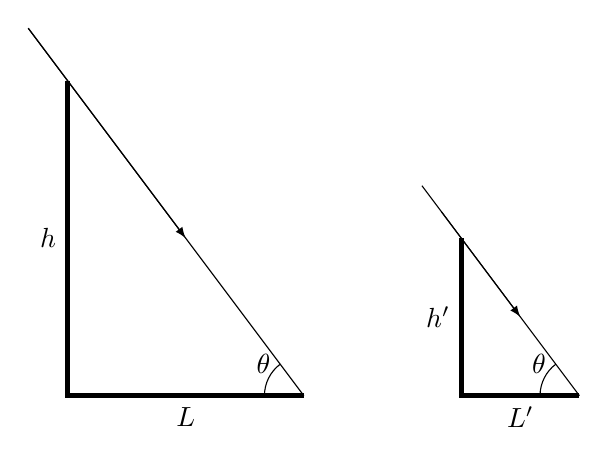
\begin{tikzpicture}[>=latex]
\begin{scope}
    \draw[ultra thick](0,4)--node[left]{$h$}(0,0)--node[below]{$L$}(3,0);
\draw(3,0)--(0,4)--(-.5,4+4/6);
\draw[->](-.5,4+4/6)--(1.5,2);
\draw(2.5,0) arc (180:126.9:.5) node[ left]{$\theta$};
\end{scope}
\begin{scope}[xshift=5cm]
    \draw[ultra thick](0,2)--node[left]{$h'$}(0,0)--node[below]{$L'$}(1.5,0);
    \draw(1.5,0)--(0,2)--(-.25,2+2/6);
    \draw[->](-.5,2+4/6)--(1.5/2,1);
    \draw(1,0) arc (180:126.9:.5) node[ left]{$\theta$};
\end{scope}
\end{tikzpicture}
    \caption{}
\end{figure}
\end{solution}

\item 边长5厘米的正方形卡片,放在小灯泡正前方15厘
米的地方,在卡片后方放一个跟卡片平行的纸屏,纸屏距卡片
15厘米,卡片在屏上的影是什么形状?面积多大?

\begin{solution}
小灯泡可视为点光源,放在卡片的正前方,屏上的影
子也是正方形的.由图5.22可知,
\[\frac{A'B'}{AB}=\frac{SQ}{SP}=\frac{15+15}{15}\]
所以,影子的边长$$A'B'=2AB=10{\rm cm}$$
影子的面积
$${A'B'}^2=10^2=100{\rm cm^2}$$
\begin{figure}[htp]
	\centering
\begin{tikzpicture}[>=latex]
\node at (-1,0)[left] {$S$};
\draw[ultra thick] (1, -.5)node[below]{$B$}--(1,.5)node [above]{$A$};
\draw (3, -2)--(3,2);
\draw (3,-1)node[below left]{$B'$}--(-1,0)--(3,1)node[above left]{$A'$};
\draw[<->] (2,.75)--(-1,0)--(2,-.75);
\draw(-1,0)--(3,0)node[right]{$Q$};
\node at (1,0) [below right]{$P$};
\fill[pattern=north east lines](3,-2) rectangle (3.2,2);
\end{tikzpicture}
	\caption{}
\end{figure}
\end{solution}

\item 在迈克耳孙测定光速的一次实验中,测得两山峰间
的距离为35373.21米,八面镜的旋转速度为528转/秒,试利
用这些数据算出光在空气中的速度.

\begin{solution}
八面镜转过八分之一转所用的时间
\[t=\frac{1}{528}\x\frac{1}{8}{\rm s}\]
光速
\[c=\frac{2s}{t}=2\x35373.21\x8\x528=2.99\x10^8\ms\]
\end{solution}

\end{enumerate}



\subsection{练习二}
\begin{enumerate}
    \item 甲乙二人面对着镜子,甲能从镜中看到乙的眼睛,乙
    是否也能看到甲的眼睛?说明理由.

    \begin{solution}
        乙能看到甲的眼睛.因为光路是可逆的.
    \end{solution}
    
    \item 在课本图5.11的潜望镜中,两平面镜倾斜的角度是多大?

    \begin{solution}
        两平面镜倾斜的角度都是$45^{\circ}$.
    \end{solution}
    
    \item 晚上在灯下看书,如果书的纸面很光滑,有时会看到
    纸面上发出刺眼的光泽,为什么会出现这种现象?怎样消除
    它?

    \begin{solution}
        光射到纸面上会同时发生镜面反射和漫反射.纸面
        越光滑,镜面反射越强.如果经光滑纸面的镜面反射的较强
        的光直接进入眼睛,就会感觉刺眼.

        改变灯光的入射方向,使得经光滑纸面的镜面反射的光
        不能直接进入眼睛,则可消除这种现象.
    \end{solution}

    \item 如课本图5.12所示,两个平面镜互相垂直,在跟这两个
    镜面垂直的平面内,有一条入射光线$AB$,经两个镜面反射后,
    沿$CD$方向射出,试证明不论光线$AB$以多大的入射角射入,反射光线$CD$都平行于$AB$射出.

    \begin{proof}
过$B$、$C$分别做镜面的法线$BN$、$CN$, 如图5.23所
示.根据反射定律,
\[\angle ABN=\angle NBC,\qquad \angle BCN=\angle NCD\]
因为两镜面互相垂直,所以
\[\angle OBC+\angle BCO=90^{\circ}\]
因此,
\[\angle NBC+\angle BCN=90^{\circ},\qquad 
\angle ABC+\angle BCD=180^{\circ}\]
所以,$AB\parallel CD$.
    \end{proof}
    \item 课本图5.13中,$M$是一个平面镜,$S$是光源,通过狭缝使
    光线射到镜面上,$M$的位置,最初是与$S$射来的光线垂直,这
    时反射光线射在标尺的零刻度上;当$M$转动一角度后,反射光
    线射到标尺的$n$刻度上.如果标尺到镜$M$的距离为$\ell$,且$\ell\gg On$,
    求$M$转动的角度是多大.
    \begin{figure}[htp]
        \centering
        \begin{minipage}[t]{0.48\textwidth}
        \centering
\includegraphics[scale=.8]{fig/5-23.png}
        \caption{}
        \end{minipage}
        \begin{minipage}[t]{0.48\textwidth}
        \centering
\includegraphics[scale=.8]{fig/5-24.png}
        \caption{}
        \end{minipage}
        \end{figure}

    \begin{solution}
        $M$转过角度$\alpha$后,镜面的法线相对于$PO$转过的角
        度也是$\alpha$, 光线$SP$经$M$反射后照到$N$(图5.24), 则
\[\angle SPN=2\alpha,\qquad \tan2\alpha=\frac{ON}{L}\] 
当$\ell\gg ON$时,$\tan 2\alpha\approx 2\alpha=\dfrac{ON}{L}$. 所以,
\[\alpha=\dfrac{ON}{L}\text{(弧度)}\]
    \end{solution}

    \item 有的镜子照出的像会变形,这是什么原因?
    
    \begin{solution}
        这是因为镜子的反射面不是理想的平面.
    \end{solution}
\end{enumerate}






\subsection{练习三}
\begin{enumerate}
    \item 有一个凹镜,要想知道它的焦距,请你想出一个粗略
        测量的方法来.

    \begin{solution}
        由于太阳光平行于主光轴,把凹镜的反射面对准太
        阳光时,光线经镜面反射后会聚于一点,这点就是焦点.测出焦点和凹镜顶点的距离,就测出了焦距.
    \end{solution}
    \item 比较凹镜和凸镜的成像情况有什么不同.

    \begin{solution}
实物通过凹镜可以成放大或缩小的倒立实像,也可
以成放大的正立虚像.

实物通过凸镜只能成缩小的正立虚像.
    \end{solution}
    \item 有一个凹镜,把它放在你的面前,如果能从镜中看到
        你自己的正立的像,这时凹镜顶点到你的距离是20厘米,那
        么这个凹镜的焦距至少有多大?

    \begin{solution}
人从凹镜中看到自己正立的像,是凹镜所成正立虚
像.这时人到凹镜顶点的距离一定小于焦距.所以凹镜的焦
距至少是20厘米.
    \end{solution}
    \item 如课本图5.18所示,$M_1$和$M_2$是两个焦距相等的凹镜,
    其焦距为$f$.要想使平行于主轴的光线$a$能在$M_1$和$M_2$之
    间来回反射,两凹镜的顶点$P_1$
    和$P_2$应相距多远?在图中标出
    两凹镜的焦点$F_1$和$F_2$的位置,
    并画出光线$a$被两凹镜反射的
    光路图.

    \begin{solution}
两凹镜的顶点$P_1$和$P_2$应相距$f$、$2f$、$3f$, 相距$2f$时
光线$a$被两凹镜反射的光路图如图5.25所示.
\begin{figure}[htp]\centering
\begin{tikzpicture}[>=latex, yscale=1.3, xscale=.8]
        \fill [pattern=north east lines] (-2,-1)--(-2.2,-1) to [bend left=30] (-2.2,1) --(-2,1) to [bend left=-30]
        (-2,-1);
\draw [thick](-2,1) to [bend left=-30] (-2,-1);
 
\fill [pattern=north east lines] (2,-1)--(2.2,-1) to [bend left=-30] (2.2,1) --(2,1) to [bend left=30](2,-1);
\draw [thick](2,1) to [bend left=30] (2,-1);
\draw [dashdotted] (-3,0)--(3,0);
\node at (-2.1,0)[below]{$P_1$};\node at (2.1,0)[below]{$P_2$};
\node at (-2.2,1)[above]{$M_1$};\node at (2.2,1)[above]{$M_2$};
\draw (-2.15,.7)--node[above]{$a$}(2.15,.7)--(-2.15,-.7)--(2.15,-.7)-- (-2.15,.7);
\node at (0,0)[above]{$F_1$};
\node at (0,0)[below]{$F_2$};
\draw[->] (-2.15,.7)--(0,.7);
\draw[->] (-2.15,-.7)--(0,-.7);
\draw[<->](-1.075,.35)--(0,0)--(-1.075,-.35);
        \end{tikzpicture}
    \caption{}
    \end{figure}
    \end{solution}
\end{enumerate}





\subsection{练习四}
\begin{enumerate}
    \item 光线以45$^\circ$的入射角从空气射入折射率为1.55的玻
璃中,折射角是多大?

\begin{solution}
    因为$\dfrac{\sin i}{\sin r}=n$
    所以,
\[r=\arcsin\left(\frac{1}{n}\sin i\right)=27.1^{\circ}\]
\end{solution}
\item 光线从空气射入水中,要想使折射角等于30$^\circ$,入射
角应为多大?

\begin{solution}
\[\sin i=n\cdot \sin r=1.33\cdot \sin 30^{\circ}=0.665\]
\end{solution}
\item 根据水和岩盐的折射率,分别算出它们中的光速,水
中的光速大约是真空中光速的几分之几?

\begin{solution}
\[\begin{split}
    v_{\text{水}}&=\frac{c}{n}=\frac{3.0\x 10^8}{1.33}=2.26\x 10^8\ms\\
    v_{\text{岩}}&=\frac{c}{n}=\frac{3.0\x 10^8}{1.54}=1.95\x 10^8\ms\\
    \frac{v_{\text{水}}}{c}&=\frac{1}{n}=\frac{2.26\x 10^8}{3.00\x 10^8}\approx \frac{3}{4}
\end{split}\]
\end{solution}
\item 课本图5.22是光线由空气进入某种媒质时的折射情况.
试由图中所给的数据求出这种媒质的折射率和这种媒质中的
光速.

\begin{solution}
\[\begin{split}
    n&=\frac{\sin i}{\sin r}=\frac{\sin(90^{\circ}-30^{\circ})}{\sin(90^{\circ}-55^{\circ})}=1.51\\
v&=\frac{c}{n}=1.99\x 10^8\ms
\end{split}\]
\end{solution}
    \item 根据上节表中给出的折射率填空:
    \begin{enumerate}
        \item 光线从水中垂直射入空气中时,折射角\underline{\qquad}
    于入射
    角;从玻璃斜射入水中时,折射角\underline{\qquad}于入射角;从空气斜射
    入酒精中时,折射角\underline{\qquad}
    于入射角;从岩盐斜射入水晶中时,
    折射角\underline{\qquad}
    于入射角.
    \item 二硫化碳比水的折射率大,由此可知二硫化碳中的光
    速比水中的光速\underline{\qquad};二者相比,二硫化碳是光\underline{\qquad}
    媒质,水是光\underline{\qquad}
    媒质.
    \end{enumerate}
    

    \begin{solution}
\begin{enumerate}
    \item 等;大;小;等.
    \item 小;密;疏.
\end{enumerate}
    \end{solution}
    \item 你在池边沿斜线向水面下看去,看到水中有一条鱼,
    你所看到的鱼的位置比实际的深还是浅?如果鱼也看到了你,
    鱼所看到的你的头的位置比实际的高还是低?

    \begin{solution}
人看到鱼的虚像$P'$位置比实际位置$P$浅,如图5.26
甲所示,鱼看到人头的虚像位置$Q'$比实际位置$Q$高,如图
5.26乙所示.
\begin{figure}[htp]
    \centering
    \includegraphics[scale=.6]{fig/5-26.png}
    \caption{}
\end{figure}
    \end{solution}
    \item 把一块厚玻璃板压在书上,透过玻璃板看书上的字
    跟拿走玻璃板直接看,感觉有什么不同?做做看,并解释看到
    的现象.

    \begin{solution}
透过玻璃板看书,看到字的虚像位置比它的实际位置高(图5.27),这是由于光通过玻璃板发生折射的缘故.
\begin{figure}[htp]
    \centering
    \includegraphics[scale=.6]{fig/5-27.png}
    \caption{}
\end{figure}
    \end{solution}
\end{enumerate}



\subsection{练习五}

\begin{enumerate}
    \item 水和金刚石的临界角各是多大?

    \begin{solution}
水对空气的临界角
\[C_{\text{水}}=\arcsin\frac{1}{n_{\text{水}}}=\arcsin\frac{1}{1.33}=48.8^{\circ}\]
金刚石对空气的临界角
\[C_{\text{金}}=\arcsin\frac{1}{n_{\text{金}}}=\arcsin\frac{1}{2.42}=24.4^{\circ}\]
    \end{solution}
    \item 课本图5.29表示一个横
截面为等腰直角三角形的玻璃
棱镜.当光从它的一个直角边垂直射入时,就从另一个直角
边垂直射出来,而没有光从斜
边射出,这种棱镜可以使光的
传播方向改变90$^\circ$.说明它的
道理.
\begin{figure}[htp]
	\centering
\begin{tikzpicture}[>=latex, scale=1.4]
  \draw (0,0)node[left]{$C$}--(2,0)node[right]{$B$}--(0,2)node[above]{$A$}--(0,0);
    \draw[ thick] (-1,1)--(1,1)--(1,-1);
\draw[->,  thick](-1,1)--(.5,1); 
\draw[->,  thick](1,1)--(1,-.5); 
\draw[dashed](.5,.5)--(1.5,1.5);
\end{tikzpicture}
	\caption{}
\end{figure}


\begin{solution}
    光垂直于界面$AC$进入玻璃棱镜中后到达界面$AB$, 入射角$i$为$45^{\circ}$(图5.28),已知玻璃对空气的折射率$n>1.5$,
    所以玻璃对空气的临界角
    \[C<\arcsin\frac{1}{1.5}=41.8^{\circ}\]
    由此可知
    $i>C$, 光在界面$AB$发生全反射,没有光线从斜边$AB$射出,光
    线垂直界面$BC$进入空气,从而使光的传播方向改变$90^{\circ}$.
\end{solution}
\item 光线从空气射入水中时,光线在水中的折射角最大为多少度?

\begin{solution}
因为$\dfrac{\sin i}{\sin r}=n$,所以
\[r=\arcsin\left(\frac{1}{n}\sin i\right)\]
当$i=90^{\circ}$时入射角最大,因此折射角的最大值为
\[r=\arcsin\frac{1}{1.33}=48.75^{\circ}\]
\end{solution}
\item 潜水的人在水面下能看到水面上的全部景象,因为
水面上180$^\circ$范围内射入水中的光线全部集中在水下97.5$^\circ$的视野内(课本图5.30),试说明它的道理.

    \begin{solution}
根据临界角的定义可知,光线从水中射向空气时发生
全反射的临界角与入射角以及折射率的关系是
\[\frac{\sin i}{\sin r}=\frac{1}{1.33}\]
所以,$i=\arcsin\left(1/1.33\right)=48.75^{\circ}$

\begin{figure}[htp]\centering
    \begin{tikzpicture}[>=latex]
    \draw(-4,2)--(4,2);
    \draw[<->](-3.5,2)--(3.5,2);
    \draw(-2.28,2)--(0,0)node[below right]{$O$}--(2.28,2);
    \draw[<->](-1.14,1)--(0,0)--(1.14,1);
    \node at (3.5,2.5){空气};
    \node at (3.5,1.5){水};
    \draw[dashdotted](0,-.5)--(0,3);
    \draw[dashed](2.28,2-1)--(2.28,2+1);
    \draw(0,.5) arc (90:41.25:.5)node[above=3pt]{$48.75^{\circ}$};
    \draw(2.28,1.5) arc (-90:-138.75:.5)node[below]{$i$};
    \end{tikzpicture}
        \caption{}
        \end{figure}

设想在水面下潜水人的眼睛处有一个点光源$O$, 由点光
源发出的光到达水面时,入射角在$0^{\circ}$—$48.75^{\circ}$(临界角)的范围
内的光都能透过水面进入空气中,相应的折射角是$0^{\circ}$—$90^{\circ}$, 
如图5.29所示.根据光路的可逆性,在水面上$180^{\circ}$范围内
的光线都能折射进入水中,到达人眼.这些光线都集中在水下
$97.5^{\circ}$的视野范围内.
    \end{solution}
\end{enumerate}



\subsection{练习六}
\begin{enumerate}
    \item 说明课本图5.31中,光线通过棱镜的$AB$和$AC$两个侧
面时,为什么都向底面偏折,如果这个棱镜的里面是空气,周
围是水,当光线通过这个空气棱镜时,射出的光线是否还向底
面偏折?画出这种情况下的光路图来.

\begin{solution}
由于棱镜玻璃的折射率$n>1$, 所以光由空气进入棱
镜时,折射角小于入射角;而光由棱镜进入空气时,是入射角
小于折射角,如图5.30所示.因此在棱镜的$AB$侧面,光由空
气进入玻璃靠近法线偏折;在$AC$侧面,光由玻璃进入空气远
离法线方向偏折.两次偏折都是偏向底面方向.
\begin{figure}[htp]
    \centering
    \includegraphics[scale=.6]{fig/5-30.png}
    \caption{}
\end{figure}

如果棱镜里面是空气周围是水,即棱镜相对于周围媒质
是光疏媒质,根据折射定律可知,当入射角$i$较小时,在$AB$
和$AC$面上的折射与上述情况相反,出射光线将向顶部方向
偏折如图5.31所示.当入射角较大时,光在$AB$侧面向顶部
方向偏折,而在$AC$侧面则可能向底部方向偏折(或不偏折),
但出射光线$GH$相对于入射光线$EF$仍然是向顶部方向偏
折,如图5.32所示.
\begin{figure}[htp]\centering
    \begin{minipage}[t]{0.48\textwidth}
    \centering
\includegraphics[scale=.6]{fig/5-31.png}
    \caption{}
    \end{minipage}
    \begin{minipage}[t]{0.48\textwidth}
    \centering
\includegraphics[scale=.6]{fig/5-32.png}
    \caption{}
    \end{minipage}
    \end{figure}
\end{solution}
\item 冕牌玻璃对紫光的折射率为1.532,对红光的折射率
为1.513.紫光和红光在这种玻璃中的速度各是多大?

\begin{solution}
因为$v=c/n$,所以
\[\begin{split}
    v_{\text{紫}} &=\frac{3.00\x 10^8}{1.532}=1.96\x 10^8\ms\\
    v_{\text{红}} &=\frac{3.00\x 10^8}{1.513}=1.98\x 10^8\ms\\
\end{split}\]
\end{solution}
\item 什么形状的全反射棱镜可以使光线改变180$^\circ$?这时
光线应从哪边射入?画出光路图来.

\begin{solution}
    等腰直角三棱镜可以使光线改变180$^\circ$. 光应垂直
    于跟直二面角相对的棱镜面射入,光路如图5.33所示.
    \begin{figure}[htp]\centering
        \begin{minipage}[t]{0.48\textwidth}
        \centering
    \includegraphics[scale=.6]{fig/5-33.png}
        \caption{}
        \end{minipage}
        \begin{minipage}[t]{0.48\textwidth}
        \centering
    \includegraphics[scale=.6]{fig/5-34.png}
        \caption{}
        \end{minipage}
        \end{figure}
\end{solution}
\item 光线通过棱镜时,偏折角度$\theta$跟棱镜材料的折射率
有关.设课本图5.31中光线对棱镜的侧面$AB$的入射角以及棱
镜的顶角$A$的大小保持不变.试定性地讨论:棱镜材料的折
射率越大,偏折角度也越大.

\begin{solution}
    光线通过棱镜发生偏折的角度为$\theta$(图5.34),
\[  \theta=(i_1-i_1')+(i_2-i_2')\]
    它表示光线通过棱镜向底面偏折的角度等于光线分别在两个
    侧面发生的向底面偏折的角度之和.在$AB$侧面,折射率$n$越
    大,从空气进入棱镜的光线向法线方向的偏折越大,即偏折角
    度$i_1-i_1'$越大;在$AC$侧面,$n$越大从棱镜射入空气的光线
    远离法线方向的偏折越大,即$i_2-i'_2$越大.因此当入射角
    以及棱镜的顶角$A$保持不变时,折射率$n$越大,偏折角度$\theta$也越大.

说明:在图5.34中,$A=i'_1+i'_2$, $\theta=i_1+i_2-A$. 又因为
\[\frac{\sin i_1}{\sin i_1'}=n,\qquad \frac{\sin i_2}{\sin i_2'}=n\]
所以
\[\sin i_1=n\sin i'_1,\qquad \sin i_2=n\sin i_2'\]
因此:
\[\begin{split}
    \sin i_2=n\sin i_2'&=n\sin (A-i'_1)\\
    &=n\left[\sin A\cos i'_1-\cos A\sin i'_1\right]\\
    &=\sin A\sqrt{n^2-n^2\sin^2 i'_1}-\cos A\sin i_1\\
    &=\sin A\sqrt{n^2-\sin^2 i_1}-\cos A\sin i_1
\end{split}\]

由上式可以明显看出,当入射角$i_1$和棱镜顶角$A$保持不
变时,折射率$n$越大,$i_2$就越大,偏折角$\theta=i_1+i_2-A$也
越大.
\end{solution}
\end{enumerate}


\subsection{练习七}
\begin{enumerate}
    \item 有一个不知焦距的凸透镜,用什么办法可以粗略地测出它的焦距?

    \begin{solution}
使太阳光沿主轴方向照到凸透镜上,在凸透镜的另
一侧可以见到一个十分亮的光点,这就是平行光会聚的焦点,
测出这一点到凸透镜的距离也就测出了凸透镜的焦距.
    \end{solution}
    \item 利用点光源和凸透镜如何能得到平行光线?

    \begin{solution}
把点光源置于凸透镜的焦点处,它发出的光经凸透
镜折射后即成平行光.
    \end{solution}
    \item 在课本图5.37中,画出光线通过透镜后的传播方向.

    \begin{solution}
        见图5.35.
\begin{figure}[htp]
    \centering
    \includegraphics[scale=.6]{fig/5-35.png}
    \caption{}
\end{figure}
    \end{solution}
\end{enumerate}





\subsection{练习八}
\begin{enumerate}
    \item 放大镜所成的像是正立、放大的,这是实像还是虚
像?放大镜应该是什么透镜?如果其焦距为$f$,镜到物的距离
最大不能超过多少?

\begin{solution}
放大镜所成的放大正立的像是虚像.放大镜应是凸
    透镜.凸透镜成放大、正立的虚像时,物距最大不能超过焦
    距,即$u<f$.
\end{solution}
\item 幻灯机所成的像是什么像?它的镜头应该是什么透
镜?如果镜头的焦距为8厘米,镜头到幻灯片的距离只能在什
么范围内变化?

\begin{solution}
    幻灯机在屏幕上所成的像是放大的倒立的实像,它
    的镜头是凸透镜,幻灯片到镜头的距离只能在$f$和$2f$之间变
    化,即$f<u<2f$, 也就是$8{\rm cm}<u<16{\rm cm}$.
\end{solution}
\item 照相机所成的像是什么像?它的镜头应该是什么透
镜?如果镜头的焦距为7.5厘米,镜头到底片的距离最短不能
小于多少?

\begin{solution}
照相机成缩小倒立实像.它的镜头是凸透镜.凸透
镜成缩小倒立实像时,$f<v<2f$, 因此底片(即像的位置)到镜
头的距离最短不能小于焦距,即7.5厘米.
\end{solution}
\end{enumerate}







\subsection{练习九}
\begin{enumerate}
    \item 如课本图5.45所示,已知物体$AB$通过凸透镜后所成的
    实像$A'B$,试画出从$A$、$B$两点射向凸透镜的任意两条光线
    $AE$、$BD$经过凸透镜折射后的传播方向.
    \begin{figure}[htp]\centering
\begin{tikzpicture}[xscale=1.5]
    \draw[<->, very thick ] (0,2)--(0,-2);
    \draw[dashdotted](-3,0)--(3,0);
\draw[->, ultra thick, >=latex] (-1,0)node[below]{$B$}--(-1,1)node[above]{$A$};

\draw[->,  thick, >=latex] (-1,0)--(0,-.5)node[below right]{$D$};
\draw[->,  thick, >=latex] (-1,1)--(0,1.2)node[right]{$E$};
\node at (.25,.25){$O$};
\draw[->, ultra thick, >=latex] (2,0)node[above]{$B'$}--(2,-2)node[below]{$A'$};
\draw[->](0,1.2)--(2,-2);
\draw[->](0,-.5)--(2,0);
\end{tikzpicture}
        \caption{}
        \end{figure}


    \begin{solution}
物点发出的光经凸透镜折射后都经过对应的像点.
从$A$点发出的光线$AE$经凸透镜折射后一定过像点$A'$, 折射
光线为$EA'$, 从$B$点发出的光线$BD$经凸透镜折射后一定过
像点$B'$, 折射光线为$DB'$, 如图5.36所示.
    \end{solution}
    \item 一物体位于凸透镜前15厘米,凸透镜的焦距为10厘
米,用作图法求出像到凸透镜的距离.

\begin{solution}
    透镜成像的光路如图5.37所示,量得$OB'=2BO$, 
    所以像到凸透镜的距离为$2\x15=30$厘米.
    \begin{figure}[htp]
        \centering
        \includegraphics[scale=.6]{fig/5-37.png}
        \caption{}
    \end{figure}
\end{solution}
\item 焦距为10厘米的凹透镜前有一物体,物到镜的距离
为20厘米,用作图法求像到镜的距离.

\begin{solution}
    透镜成像光路如图5.38所示.量得物距$BO$为像
    距$B'O$的3倍,所以像到凹透镜的距离为$\dfrac{20}{3}=6.7$厘米.
    \begin{figure}[htp]
        \centering
        \includegraphics[scale=.6]{fig/5-38.png}
        \caption{}
    \end{figure}
\end{solution}
\item 在课本图5.46中,$OO'$为透镜的主轴,$A'B'$为物体$AB$
经透镜所成的像.这个透镜是什么透镜?试用作图法求出透
镜和它的焦点的位置.                    

    \begin{solution}
由题可知,像$A'B'$是物$AB$的倒立实像,所以透镜是
凸透镜.成像光路图、透镜位置以及焦点位置,如图
5.39所示.
\begin{figure}[htp]\centering
    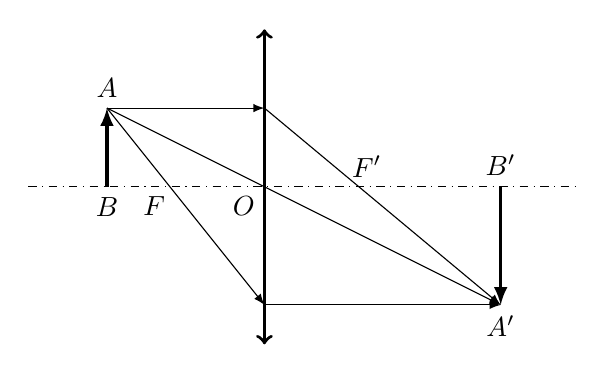
\begin{tikzpicture}
        \draw[<->, very thick ] (3,2)--(3,-2);
\draw [dashdotted](0,0)--(7,0);
\draw [->, very thick, >=latex](1,0)node[below]{$B$}--(1,1)node[above]{$A$};
\draw [->, very thick, >=latex](6,0)node[above]{$B'$}--(6,-1.5)node[below]{$A'$};

\draw[->, >=latex](1,1)--(3,1);  \draw[->, >=latex](3,1)--(6,-1.5);
\draw[->, >=latex](1,1)--(3,-1.5);  \draw[->, >=latex](3,-1.5)--(6,-1.5);
\draw[->, >=latex](1,1)--(6,-1.5);
\node at (4.3,0)[above]{$F'$};
\node at (1.6,0)[below]{$F$};
\node at (3,0)[below left]{$O$};

    \end{tikzpicture}
    \caption{}
    \end{figure}
    \end{solution}
\end{enumerate}





\subsection{练习十}

\begin{enumerate}
    \item 试证明:
$\dfrac{1}{u}+\dfrac{1}{v}=\dfrac{1}{f}$也
适用于凹透镜成像.(提示:
对于凹透镜$f$和$v$应取负值)

\begin{proof}
    物体经凹透镜成缩小虚像,光路如图5.40所示.焦
距$f$和虚像像距$v$都是负值.用$-f$和$-v$分别表示图中的
几何线段$FO$和$B'O$的大小.
    \begin{figure}[htp]
        \centering
        \includegraphics[scale=.6]{fig/5-40.png}
        \caption{}
    \end{figure}
    
因为$\triangle OA'B\backsim \triangle OAB$, 所以
\[\frac{OB'}{OB}=\frac{A'B'}{AB},\qquad \frac{-v}{u}=\frac{y'}{y}\]
又因为$\triangle F'A'B'\backsim \triangle FEO$, 所以
\[\frac{F'B'}{F'O}=\frac{F'O-B'O}{F'O}=\frac{A'B'}{AB}\]
即\[\frac{(-f)-(-v)}{(-f)}=\frac{y'}{y}\]
因此:
\[\frac{-v}{u}=\frac{v-f}{-f}\]
即$fv=uv-uf$. 整理后得
\[\frac{1}{u}+\frac{1}{v}=\frac{1}{f}\]
\end{proof}
\item  利用公式
$\dfrac{1}{u}+\dfrac{1}{v}=\dfrac{1}{f}$,
试讨论:
\begin{enumerate}
    \item 对于凸透镜,物距$u$在什么范围内变化时,$v$为正值,
    成实像?在什么范围内变化时,$v$为负值,成虚像?
    \item 对于凹透镜,$v$能否为正值?
\end{enumerate}

\begin{solution}
    \begin{enumerate}
        \item 由$\dfrac{1}{u}+\dfrac{1}{v}=\dfrac{1}{f}$,可得
    \[v=\frac{u\cdot f}{u-f}\]
    实物通过凸透镜成像,$u>0$, $f>0$.
    \begin{itemize}
        \item     当$u-f>0$,即 $u>f$时,$v>0$成实像.
        \item  当 $u-f<0$,即$u<f$时,$v<0$成虚像.
    \end{itemize}
\item 由于实物通过凹透镜成像时,$u>0$, $f<0$, 所以总有
    $u\cdot f<0$, $u-f>0$. 因此
    \[v=\frac{u\cdot f}{u-f}<0\]
    即$v$不能为正值.
    \end{enumerate}
\end{solution}
\item 一支蜡烛,距凸透镜24厘米,在离凸透镜12厘米的
屏上得到清晰的像.这个凸透镜的焦距是多长?像是放大的
还是缩小的?画出成像光路图.

\begin{solution}
\[\begin{split}
    f&=\frac{u\cdot v}{u+v}=\frac{24\x 12}{24+12}=8{\rm cm}\\
    m&=\frac{v}{u}=\frac{12}{24}=\frac{1}{2}
\end{split}\]
像是缩小的实像,成像光路图如图5.41所示.
\begin{figure}[htp]
    \centering
    \includegraphics[scale=.6]{fig/5-41.png}
    \caption{}
\end{figure}
\end{solution}
\item 照相机的镜头相当于一个凸透镜,如果镜头的焦距
为10厘米,底片长3.6厘米,要想给身高1.8米的人拍一张全
身像,人到镜头的距离至少为多少米?

\begin{solution}
\[m'=\frac{A'B'}{AB}=\frac{3.6\x 10^{-2}}{1.8}=2\x 10^{-2}\]
将数值代入$m=v/u$和$\dfrac{1}{v}+\dfrac{1}{u}=\dfrac{1}{f}$
两公式,可得
\[\begin{cases}
    \dfrac{v}{u}=2\x 10^{-2}\\
    \dfrac{1}{u}+\dfrac{1}{v}=\dfrac{1}{10{\rm cm}}
\end{cases}\]
解得$u=5.1$米.

为了照全身像,人到镜头的距离至少为5.1米.
\end{solution}
\item 用焦距为10厘米的凸透镜作放大镜来看微小的物
体,要想使像成在离镜25厘米的地方,镜到物的距离应为多
少?这时看到的像放大了多少倍?

\begin{solution}
用凸透镜作放大镜时成的是虚像,所以$v$为$-25$厘
米.由透镜成像公式可得
\[\frac{1}{u}+\frac{1}{-25{\rm cm}}=\frac{1}{10{\rm cm}}\]
得到$u=7.1$厘米.

因此,
\[m=\left|\frac{v}{u}\right|=\frac{25}{7.1}=3.5\]
\end{solution}
\item 物体位于离凹透镜15厘米处,凹透镜的焦距是7.5
厘米,像距是多大?像的放大率是多大?

\begin{solution}
    凹透镜的焦距$f=-7.5$厘米,代入透镜成像公式
    可得
\[\frac{1}{15{\rm cm}}+\frac{1}{v}=\frac{1}{-7.5{\rm cm}}\quad \Rightarrow\quad v=-5{\rm cm}\]
\[m=\frac{|v|}{u}=\frac{5}{15}=\frac{1}{3}\]
\end{solution}
\item 幻灯机的镜头也相当于一个凸透镜,如果不改变幻
灯机的镜头,当幻灯机到幕的距离增大时,应该怎样调节镜头
到幻灯片的距离,才能得到清晰的像?这时幕上的像是变大还
是变小?

\begin{solution}
    幻灯片通过镜头成放大实像,一般来说镜头到屏幕
    的距离(像距)远远大于幻灯片到镜头的距离(物距),因此幻
    灯机到幕的距离可以当作像距$v$. 由透镜公式可知,镜头焦
    距$f$不变,$v$增大时,$u$必定减小,即应使镜头靠近幻灯片,才
    能得到清晰的像.由公式$m=v/u$
    可知,$v$增大而$u$减小时,$m$
    将增大,屏上的像变大.
\end{solution}
\end{enumerate}





\subsection{习题}
\begin{enumerate}
    \item 为了使身高1.8米的人能从平面镜中看到自己的全
身像,如果镜和人都是直立的,平面镜的长度至少应为多长?
画图加以说明.

\begin{solution}
如图5.42所示.人 
身高$AB=1.8$米,对于平面镜
$MN$人与像是对称的,像长$A'B'=1.8$米.人如果能从镜中
看到自己的全身像,必须使$AB$各点发出的光通过镜面$MN$
反射后都能到达人眼$C$处,即好象是从虚像$A'B'$发出的光都
到达$C$点.$CA'$、$CB'$与镜面的交点是$P$、$Q$,$PQ$的长度就是平
面镜的最小长度.
\begin{figure}[htp]
    \centering
    \includegraphics[scale=.6]{fig/5-42.png}
    \caption{}
\end{figure}

由于$AB$、$MN$都是直立的,有$AB\parallel MN\parallel A'B'$. 所以$\triangle CPQ\backsim \triangle CA'B'$. 根据
\[\frac{PQ}{A'B'}=\frac{CP}{CA'}=\frac{1}{2}\]
所以
\[PQ=\frac{1}{2}A'B'=0.90{\rm m}\]
\end{solution}
\item 光可以从弯曲玻璃棒的一端传到另一端,这是否跟
光在同一种媒质中沿直线传播相矛盾?

\begin{solution}
    不矛盾.光从玻璃棒的一端射入,在均匀玻璃棒内
    是沿直线传播的.在玻璃和空气的界面处发生全反射后,在
    玻璃棒内继续沿直线传播.光在玻璃和空气界面处多次发生
    全反射,才使光沿着折线从弯曲的玻璃棒的一端传到另一端.
\end{solution}
\item 在水面下1.0米处有一个点光源,从水面上看,这个
点光源能照亮水面多大的面积?

\begin{solution}
    有折射光线射出的水面,才是在水面上看到的光源
    照亮的面积.由于水对空气的临界角
\[    C=\arcsin\frac{1}{n}=48.8^{\circ}\]
    也就是在图5.43中,$\angle SAN=48.8^{\circ}$, 光的入射角大于$48.8^{\circ}$的水面,没有折射光线射出.所以从水面上看,被这个点光源
    照亮的面积为以$O$为圆心$OA$为半径的圆.

    因为
    \[OA=h\cdot \tan C=1.0\x\tan48.8^{\circ}=1.14{\rm m}\]
    所以圆面积
    \[S=\pi\cdot (OA)^2=3.14\x1.14^2=4.08{\rm m^2}\]
\end{solution}

\begin{figure}[htp]\centering
    \begin{minipage}[t]{0.48\textwidth}
    \centering
\includegraphics[scale=.7]{fig/5-43.png}
    \caption{}
    \end{minipage}
    \begin{minipage}[t]{0.48\textwidth}
    \centering
\includegraphics[scale=.7]{fig/5-44.png}
    \caption{}
    \end{minipage}
    \end{figure}

\item 用下面的方法可以测量液体的折射率:取一个半径
为$r$的软木塞,在它的圆心处插上一枚大头针,让软木塞浮在
液面上(课本图5.58).调整大头针插进软木塞的深度,使它露在
外面的长度为$h$.这时从软木塞周围各个方向向液体中看,恰
好看不到大头针.利用测得的数据$r$和$h$即可以求出液体的
折射率.
\begin{enumerate}
    \item 写出用$r$和$h$求折射率的计算式;
    \item 用这种方法实际做一下,求出水的折射率.
\end{enumerate}

\begin{solution}
    在图5.44中,$P$为大头针的顶部,$A$为软木塞边缘
某点,$AN$为法线.在液面上从各个方向向液体中恰好看不
到大头针时,$\angle PAN=C$(临界角).

因为    
\[AP=\sqrt{r^2+h^2},\qquad \sin C=\frac{r}{\sqrt{r^2+h^2}},\qquad \sin C=\frac{1}{n}\]
所以
\[n=\frac{1}{\sin C}=\frac{\sqrt{r^2+h^2}}{r}\]
\end{solution}


\item 为了从坦克内部观察外界目标,在坦克壁上开有一
个长方形孔.假定坦克的壁厚为20厘米,孔的宽度为12厘
米,孔内安装一块折射率$n=1.52$的玻璃,厚度跟坦克的壁厚
相同,车内人员通过这块玻璃能看到的外界范围为多大角度?

\begin{solution}
    外界的光通过玻璃到达处于孔中心处$P$点的人眼
    (图5.45)时,
\[\sin i=n\cdot \sin r=1.52\x \frac{6.0}{6^2+20^2}=0.44\quad \Rightarrow\quad i=26^{\circ}\]
眼在中心处观察可以看到外界范围的角度为$2i=52^{\circ}$.
\begin{figure}[htp]\centering
    \begin{minipage}[t]{0.48\textwidth}
    \centering
\includegraphics[scale=.7]{fig/5-45.png}
    \caption{}
    \end{minipage}
    \begin{minipage}[t]{0.48\textwidth}
    \centering
\includegraphics[scale=.7]{fig/5-46.png}
    \caption{}
    \end{minipage}
    \end{figure}

说明:
人眼在不同位置观察时,看到外界的范围是不同的.当
人眼P位于孔的边缘处观察图5.46, 可得
\[\sin i=n\cdot \sin r =1.52\x \frac{12}{\sqrt{20^2+12^2}}=0.78\quad \Rightarrow\quad i=51^{\circ}\]
观察范围(角度)为$51^{\circ}$.

\end{solution}
\item 课本图5.59中给出了光线在光学器件上射入和射出的
方向,试在方框内画出可用的光学器件及光路图.

\begin{solution}
    答案如图5.47所示.
    \begin{figure}[htp]
        \centering
        \includegraphics[scale=.7]{fig/5-47.png}
        \caption{}
    \end{figure}
\end{solution}
\item 如果把凸透镜的中部用一块黑纸遮住,用它还能得
到物体的像吗?为什么?

\begin{solution}
凸透镜成像是由于光在透镜两侧界面上发生折射的
结果.如果凸透镜中部用一块黑纸遮住,它的其余部分仍能
透过光线,并在两侧界面上发生折射,仍能成像.只是由于黑
纸的遮挡,透过凸透镜的光减少了,成像的亮度降低.
\end{solution}
\item 蜡烛到凸透镜的距离为20厘米,到光屏的距离为40
厘米,这时在光屏上得到清晰的烛像,如果把凸透镜向光屏
移动5厘米,光屏应向后移动多远才能再得到清晰的烛像?这
时像的放大率是增大了,还是减小了?

\begin{solution}
    \begin{figure}[htp]
        \centering
        \includegraphics[scale=.7]{fig/5-48.png}
        \caption{}
    \end{figure}

    在图5.48中,物距$u=20$厘米,像距$v=L-u=40-20=20$厘米.
    焦距
\[f=\frac{uv}{u+v}=\frac{20\x 20}{20+20}=10{\rm cm}\]
\[m=\frac{v}{u}=1\]

将凸透镜向光屏移动$d=5$厘米,物距$u'=u+d=25$
厘米,像距
\[v'=\frac{u'f}{u'-f}=\frac{25\x 10 }{25-10}=17{\rm cm}\]
光屏移动的距离
\[\Delta L=u'+v'-L=2{\rm cm}\]
放大率$m'=\dfrac{v'}{u'}=\dfrac{17}{25}=0.68<m$, 像的放大率减小了.
\end{solution}
\item 当物体到凸透镜的距离为36厘米时,光屏上所成的
像的高度为10厘米;当物体到凸透镜的距离变为24厘米时,
光屏上像的高度变为20厘米,这个凸透镜的焦距是多大?

\begin{solution}
    由透镜公式$\dfrac{1}{u}+\dfrac{1}{v}=\dfrac{1}{f}$
    和放大率公式$m=\dfrac{v}{u}=\dfrac{y'}{y}$($y$和$y'$分别为物和像的高度)可得
\[f=\frac{u\cdot v}{u+v}=\frac{mu}{m+1}=\frac{y'\cdot u}{y'+y}\]
则
\[f=\frac{y'_1\cdot u_1}{y'_1+y},\qquad f=\frac{y'_2\cdot u_2}{y'_2+y}\]
消$y$并代入数值得
\[f=\frac{y'_1u_1-y'_2u_2}{y'_1-y'_2}=\frac{10\x 36+20\x 24}{10-20}=12{\rm cm}\]
\end{solution}
\item 透镜焦距的倒数$1/f$
叫做透镜的焦度,焦度的单位叫
做屈光度,透镜的焦距为1米时,焦度为1屈光度.屈光度
乘以100,就是通常所说的眼镜的度数,某同学眼镜的近视度
数是250度,他的眼镜是什么透镜?焦距是多大?

\begin{solution}
    近视眼镜为凹透镜.
    
    250度近视镜的焦度
\[D=\frac{-250}{100}=-2.5\text{屈光度}\]
\[f=\frac{1}{D}=-\frac{1}{2.5}=-0.40{\rm m}=-40{\rm cm}\]
\end{solution}
\item 如图5.49所示,如果以凸透镜的两个焦点$F_1$、$F_2$
分别作为计算物距和像距的起点,并且用$x$表示物体$AB$到
第一焦点$F_1$的距离,以$x'$表示像$A'B'$到第二焦点$F_2$的距
离.试证明;凸透镜成像的公式
\[\frac{1}{u}+\frac{1}{v}=\frac{1}{f} \]
将变为$xx'=f^2$.此式称为牛顿薄透镜公式,在光学书中经常遇到.
\begin{figure}[htp]
	\centering
\begin{tikzpicture}
  \draw [dash dot](-4,0)--(5,0);
\fill (-2,0) circle (1.5pt) node[below]{$F_1$};
\fill (2.5,0) circle (1.5pt)node[above]{$F_2$};
\draw[->, very thick, -latex](-3.5,0)node[below]{$B$}--(-3.5,.8)node[above]{$A$};
\draw[->, very thick, -latex](4.5,0)node[above]{$B'$}--(4.5,-1.5)node[below]{$A'$};
\draw[<->, ultra thick ](0,2)--(0,-2);
\node at (.25,.25){$O$};
\draw[ stealth-stealth](-3.5,.4)--node [fill=white]{$x$}(-2,.4);
\draw[ stealth-stealth](4.5,-.4)--node [fill=white]{$x'$}(2.5,-.4);
\draw (-2,0)--(-2,.5); \draw (2.5,0)--(2.5,-.6); 
\end{tikzpicture}
	\caption{}
\end{figure}
(提示:$u=x+f$,$v=x'+f$)

\begin{proof}
在$\dfrac{1}{u}+\dfrac{1}{v}=\dfrac{1}{f}$公式中代入$u=x+f$、$v=x'+f$, 
得到
\[\frac{1}{x+f}+\frac{1}{x'+f}=\frac{1}{f}\]    
整理可得
\[x'f+xf+2f^2=xx'+fx'+xf+f^2\]
所以$x\cdot x'=f^2$

注意:牛顿公式也可由透镜成像作图(图5.50)直接
证明.
\begin{figure}[htp]
    \centering
    \includegraphics[scale=.7]{fig/5-50.png}
    \caption{}
\end{figure}

因为$\triangle FAB\backsim \triangle FDO$, 所以
$\dfrac{AB}{DO}=\dfrac{x}{f}$,
又因为$\triangle F'A'B'\backsim \triangle F'CO$, 所以$\dfrac{CO}{A'B'}=\frac{f}{x'}$
而$AB=CO$, $A'B'=DO$, 因此
\[\frac{x}{f}=\frac{f}{x'},\qquad x\cdot x'=f^2\]
\end{proof}
\item 某人用焦距为2厘米和8厘米的两个凸透镜分别
作物镜和目镜,制成一架简易显微镜.如果物镜到被观察物
体的距离为2.2厘米,要想使目镜最后所成的虚像距目镜25
厘米,目镜和物镜间的距离应为多大?这架显微镜的放大率是
多大?

\begin{solution}
对于目镜成放大的虚像,像距 $v_2=-25$厘米,
$f_2=8$厘米.对应的物距
\[u_2=\frac{f_2\cdot v_2}{v_2-f_2}=\frac{8\x (-25)}{-25-8}=6.1{\rm cm}\]
对于物镜成放大实像.物距$u_1=2.2$厘米,$f_1=2$厘米.
对应的像距
\[v_1=\frac{f_1\cdot u_1}{u_1-f_1}=\frac{2\x 2.2}{2.2-2}=22{\rm cm}\]
所以目镜和物镜间的距离$L=v_1+u_2=28$厘米
显微镜的放大率
\[m=m_1\cdot m_2=\frac{v_1}{u_1}\cdot \frac{v_2}{u_2}=\frac{22}{2.2}\x\frac{25}{6.1}=41\]
光路图如图5.51所示.
\begin{figure}[htp]
    \centering
    \includegraphics[scale=.7]{fig/5-51.png}
    \caption{}
\end{figure}
\end{solution}
\end{enumerate}
























\section{参考资料}
\subsection{光的速度}
光速是在物理学史和科学技术上有着非常重要意义的基
本物理常数.

1851年傅科测出水中的光速小于真空中的光速,成为波
动说战胜微粒说的实验依据.

1865年麦克斯韦从理论上计算出电磁波速度
\[v=\frac{1}{\sqrt{\varepsilon_0\cdot \mu_0}}=
3.10740\x10^5{\rm km/s}\]
与实验测定的光速值一致,他大胆地预言光是一种电磁波,建
立了光的电磁学说.

真空中光速的测量为狭义相对论的建立奠定了实验基
础.真空中光速恒定不变,不管选择什么样的参照系,也不管
光源或接收器是否运动.光速不变原理成为狭义相对论的基
本假设之一.

本世纪70年代以后,光速的测量已十分精确,以致在
1983年第十七届国际计量大会上决定,用光速重新定义长度
的基准单位——米:“米”是光在真空中,在$1/299792458$秒的
时间间隔内运行路程的长度.

测量真空中的光速一览表
\begin{center}
    \begin{tabular}{lp{.3\textwidth}p{.3\textwidth}l}
\hline
年代&作者&方法&光速值(km/s)\\
\hline
1727年&布喇德雷(Bradley)&光行差法& $301,000$\\
1849年&斐索(Fizeau)&齿轮法& $313,000$\\
1851年&傅科(Foucault)&旋转镜法& $298,000\pm 500$\\
1933年&迈克耳孙(Michelson)皮斯(Pease)皮尔孙(Pearson)   &旋转镜法& $299,774\pm 2$\\
1941年&安德森(Anderson)&克尔盒调谐器&$299,776\pm 6$\\
1950年&埃森(Essen)&谐振腔法&$299,792.5\pm 1$\\
1951年&贝格斯特兰(Bergstrand)&光电测距仪&$299,793.1\pm 0.3$\\
1956年&艾奇(Edge)&光电测距仪&$299,792.2\pm 0.1$\\
1957年&韦德莱(Wadley)&雷达测距仪&$299,792.6\pm 1.2$\\
1958年&弗罗默(Froome)&微波干涉仪&$299,792.5\pm 0.1$\\
1961年&卡特科斯基(Cutkosky)托马斯(Thomas)&电荷的静电单位和电磁单位的比值&$299,791.96\pm 0.8$\\
1964年&
兰克、琼斯、艾迪(Rank, Jones, Gordy)&光谱法(氯化氢)&$299,792.8\pm 0.4$\\
1966年&卡洛路斯、赫姆伯格(Karolus, Helmberger)&声调制法&$299,792.47\pm 0.15$\\
1972年&贝依等(Bay)&氦氖激光(0.663微米)&$299,792.462\pm 0.018$\\
1972年&贝艾德(Baird)&二氧化碳激光(9和10微米)&$299,792.460\pm 0.006$\\
1973年&美国国家标准局&测定氦-氖激光3.39微米谱线的频率和波长&$299,792.574\pm 0.0011$\\
1974年&美国国立物理实验室&测定$\rm CO_2$激光9.3微米谱线的频率和波长&$299.792.4590\pm 0.0008$\\
\hline
    \end{tabular}
\end{center}


\subsection{光导纤维}

从20世纪50年代开始利用光导纤维传输光能的技术得
到迅速发展.至今已经形成一门专门的科学——纤维光学.
根据传输光能的机制,光导纤维可以分为反射型和折射型
两类.

反射型光导纤维由两层均匀媒质组成(图5.52甲),内层
称为芯线,外层称为包层,芯线的折射率$n_1$大于包层的折射
率$n_2$. 光从圆柱形光导纤维端面入射,进入芯线内传播,到达
芯线与包层的界面处发生全反射(图5.52乙),使得光只在芯
线中由一端传到另一端而不进入包层,光能量的损失较小.
\begin{figure}[htp]\centering
\includegraphics[scale=.6]{fig/5-52.png}
    \caption{}
    \end{figure}

折射型光导纤维是折射率非均匀分布的光导纤维.光导
纤维的折射率在它的横断面上沿半径方向连续变化,中心轴
线处折射率最大,沿半径向外逐渐减小(图5.53甲),在光导纤
维内部,光传播的径迹总是偏向中心轴线方向弯曲的周期性
变化的曲线,如(图5.53乙)所示.和反射型光导纤维一样,光
从端面射入光导纤维内传播时,也约束在光导纤维内部一
定范围内.折射型光导纤维还具有自动聚焦作用.以不同角
度入射到$O$点的光线在光导纤维内行进半个周期的整数倍的
路程后,还可以交于一点.光导纤维对光的这种作用和透镜
对光的作用一样,因此,可以用在成像系统中.
\begin{figure}[htp]\centering
    \includegraphics[scale=.6]{fig/5-53.png}
        \caption{}
        \end{figure}

光导纤维被广泛地用于传输光能,具有结构简单、可以任
意弯曲的优点.在医疗上,光导纤维可以用于照明和成像,把
光导纤维伸入人体内,强光源的光聚焦到光导纤维的注入面,
光通过光导纤维传送到人体内,照亮病人体内的病灶部位.同
时,再由光导纤维把病变的图象传送出来,供医生观看.如果
把能量足够高的激光通过光导纤维传输到人体内,还可以完
成高效的外科手术.女果用光导纤维把激光能量传输到体内
出血部位,用激光的凝血作用止血,可治疗胃溃疡病人内
出血.

光导纤维和激光技术相结合,发展为光纤通信.光纤通
信用光导纤维作传输信号的媒质,用光波作载波.传输的任
何信息或由信息转换成的交变电流都有一定的频率范围,称
为频带宽度,简称带宽.载波要能携带信息,其频带必须比
信息的频带更宽.人发出的声音的频带为0.3千赫—3.4千
赫,如果传输一路电话,载波的频带宽度须大于3.4千赫.
所以载波的频带越宽,所能传输的通话路数越多.光纤通信
用光波作为载波,光的频率在$10^{10}$—$10^{12}$千赫,可同时容纳
100亿个话路.

在传输信号的媒质上也存在着带宽的问题.由它限制着
所能传输的信号的频带宽度.对光纤来说,由它的色散特性
决定了它所允许的传输带宽很宽.

通常电话信号占用的频带为4—5千赫,彩色电视信号占
用频带宽约8—10兆赫.利用光波做载波的光纤通信技术,目
前已能在一根光导纤维上传送几万路电话或者几十路电视.
在实际中,还常常用几对、几十对乃至几百对光导纤维组成光
缆,这样,使每根光缆的通信容量又可以增加几倍,甚至几百
倍.另外,光纤通信的中继距离长.在微波通信线路中,由于电
波能量的损耗,每隔一段路程就要设置中继站,把接收到的电
波信号放大,才能继续传播下去.对于微波通信,中继站的间
隔为3公里.对于光纤通信,由于制造光纤的技术不断改进,
1970年美国制造的光导纤维每公里衰减20分贝(即每公里衰
减到原来的1/100),现在生产的光导纤维每公里只衰减0.2
分贝,非常接近于理论的极限值0.18分贝.这样,光纤通信
的中继站的间距可以大大拉长,目前可达到100公里以上,此
外,光纤通信还具有线径小(一根光纤的直径为0.06—0.1毫
米)、重量轻,(现在的轻质光缆每公里不到2千克),取材易、
价格低廉,抗干扰、耐震动等优点,到1983年底,全世界共
敷设27万公里长的光纤通信线路,我国在上海、北京、武汉等
城市中敷设了总长100多公里的光纤通信线路,连接武汉三
镇的光纤电话已通过鉴定,并已在试用.我国新兴的光纤通
信产业已初具规模,在一些重要技术上已达到国际八十年代
初的水平.

\subsection{助视光学仪器的视角放大倍数}
助视光学仪器包括放大镜、显微镜和望远镜.使用助视
光学仪器的主要目的是放大视角,通常用视角放大倍数来衡
量助视光学仪器的放大本领.物体通过助视光学仪器得到的
虚像对人眼所张的视角$U'$与物体直接对人眼所张的视角$U$
之比,即$M=U'/U$
叫做光学仪器的视角放大倍数.视角越大.
物体在视网膜上所成的实像也越长.在近轴条件下,
\[U\approx \sin U\approx \tan U, U'\approx \sin U'\approx \tan U'\]
因此,视角放大倍数也等
于借助于助视光学仪器后物体在视网膜上所成的实像长$h'$
与物体直接在视网膜上所成实像长$h$之此.即
\[M=\frac{U'}{U}=\frac{h'}{h}\]

(1)放大镜用来观察近处比较细小的物体,最简单的放
大镜是一个凸透镜.它的放大倍数计算如下:

眼睛直接观察,细小物体,一般放在明视距离$L=25$厘米
处.视角$U=y/L$(图5.54甲).

\begin{figure}[htp]\centering
    \includegraphics[scale=.6]{fig/5-54.png}
        \caption{}
        \end{figure}

眼睛通过放大镜观察,看到的是细小物体的放大虚像,视
角$U'=y'/L'$(图5.54乙),其中$L'=-x'+X'$, 代入放大率
公式
\[m=\frac{y'}{y}=-\frac{x'}{f}\]
视角放大倍数
\[\begin{split}
    M=\frac{U'}{U}=\frac{y'}{y}\cdot \frac{L}{L'}&=-\frac{x'}{f}\cdot \frac{25}{L'}{\rm cm}\\
    &=\frac{25}{f}{\rm cm}\x \left(1-\frac{X'}{L'}\right)
\end{split}\]
一般说来,放大镜的放大本领与放大镜的焦距有关,还与放大
镜的使用情况,即物和透镜的距离,人眼和透镜的距离有关.
当人眼处于像方焦点$F'$处时,$X'=0$, 则
\[M_0=\frac{25}{f}\]
仅与放大镜的焦距有关,一般所说的放大镜的放大倍数就是
指$M_0$来说的.

由于像差的存在,一般简单放大镜的放大倍数不超过
3倍.

\begin{figure}[htp]\centering
    \includegraphics[scale=.6]{fig/5-55.png}
        \caption{显微镜成像光路}
        \end{figure}

(2)显微镜由焦距很短的物镜和焦距较长的目镜组成.
其成像光路如图5.55所示.近处细微的物体放在物镜的物方
焦平面附近,成倒立实像于目镜的物方焦面附近,从目镜折射
出来的光线都近于平行,这样,虚像$y'$对人眼张的视角$U'$近
似等于实像$y_1$对目镜光心$O_2$所张的角度.即$U'=y_1/f_2$. 
由于
物镜的放大率
\[m_1=\frac{y_1}{y}=\frac{V_1}{u_1}\]
对物镜来说,物距$u_1$近似等于它
的焦距$f_1$, 像距$v_1$近似等于镜筒长$L$, 所以
\[\frac{y_1}{y}\approx \frac{L}{f}\]
由此得到
\[U'=\frac{y\cdot L}{f_1\cdot f_2}\]

直接将物体放在明视距离处观察的视角$U=\dfrac{y}{25{\rm cm}}$
微镜的视角放大倍数
\[M=\frac{25{\rm cm}}{f_2}\cdot \frac{L}{f_1}\]
相当于目镜的放大倍数和物镜的放大倍数的乘积.通常显微镜的目镜和物镜都标有
放大倍数的字样,如物镜标有$40\x$, 目镜标有$15\x$, 则它们组
成的显微镜的放大倍数是$M=40\x15=600$(倍).

(3)望远镜用来观察远处大物体.由于物体距人眼很远,
视角很小,难以被人分辨清楚.望远镜的作用就是放大视角,
物体通过望远镜成虚像,该虚像对人眼所张的视角比物体直
接对人眼所张的视角大,犹如把物体从远处“拉近”一样.

开普勒望远镜的目镜和物镜都是凸透镜,物镜的焦距$f_1$
大于目镜的焦距$f_2$, 它们相距$L=f_1+f_2$, 因此物镜的像方焦
平面和目镜的物方焦平面重合.远处的物体$AB$通过物镜成
实像$A_1B_1$于焦平面上,再通过目镜或虚像于无限远处.该虚
像对人眼所张的视角等于像$A_1B_1$对目镜光心$O_2$张的角度
\[U'=\frac{y'}{f_2}\]
远处物体直接对人眼所张的视角等于它对物镜的光心$O_1$所
张的视角$U$, 由图5.56可以看出,$U=y'/f_1$.
望远镜的视角放大
倍数为$M=f_1/f_2$.

\begin{figure}[htp]\centering
    \includegraphics[scale=.6]{fig/5-56.png}
        \caption{开普勒望远镜成像光路}
        \end{figure}

